% Author Name: José Areia 
% Author Contact: jose.apareia@gmail.com
% Version: 2.2.13 - 2026/01/06
% Public Repository: https://github.com/mfrade/ULO-thesis
% Getting Help: https://github.com/mfrade/ULO-thesis/issues
% Forked From: https://github.com/joseareia/ipleiria-thesis

%%% Document Options %%%
\documentclass[
    language=english,
    school=estg,
    docstage=final,
    media=paper,
    bookprint=false,
    linkcolor=red!45!black,
    chapterstyle=classic,
    coverstyle=bw,
    aiacknowledgement=true,
    listprefix=false
]{ULOThesis} % Refer to the Wiki for a list of available options.

%%% Document Version %%%
\DocumentVersion{1.0.0} % Required only if the 'docstage' is set to 'working'.

%%% Document Metadata %%%
% First Author (Mandatory)
\FirstAuthor{Igor Ferreira do Nascimento}
\FirstAuthorNumber{2240253}

% Second Author (Optional)
% \SecondAuthor{Jane Smith}
% \SecondAuthorNumber{2230456}

% Third Author (Optional)
% \ThirdAuthor{July Smith}
% \ThirdAuthorNumber{2230457}

% Supervisor (Mandatory)
\Supervisor{João da Silva Pereira}
\SupervisorMail{joao.pereira@ipleiria.pt}
% Please provide: [Current Title, Affiliation]
\SupervisorTitle{Full Professor, Polytechnic of Leiria} 

% % Co-Supervisor (Optional)
% \CoSupervisor{}
% \CoSupervisorMail{}
% \CoSupervisorTitle{}

% % Second Co-Supervisor (Optional)
% \SecCoSupervisor{}
% \SecCoSupervisorMail{}
% \SecCoSupervisorTitle{}

% Title (Mandatory)
\Title{SBOM Lens: A Graph-Based Framework for Software Supply Chain Risk Assessment}

% Subtitle (Mandatory)
\Subtitle{Structural Metrics and Network Topology Analysis of Software Dependency Networks}

% University (Mandatory)
\University{Polytechnic of Leiria}

% School (Mandatory)
\School{School of Management and Technology}

% Department (Mandatory)
\Department{Department of Computer Engineering}

% Degree (Mandatory)
\Degree{Master in Cybersecurity \& Digital Forensics}

% Course (Optional)
% \Course{Offensive \& Defensive Cybersecurity}

% Thesis Theme (Mandatory)
\ThesisType{Project}

% Local & Date (Mandatory)
\Date{Leiria, \DTMmonthname{\month} \number\year}

% Academic Year 
\AcademicYear{2025/26}

%%% Application Screenshots %%%
% \screenshot[width]{Figures/<path> without .png}{what to capture}
% Shows the PNG once it exists; until then, a framed box saying what to capture.
\newcommand{\screenshot}[3][\textwidth]{%
    \IfFileExists{#2.png}{%
        \includegraphics[width=#1]{#2.png}%
    }{%
        \fbox{\parbox[c][0.45\linewidth][c]{\dimexpr #1 - 2\fboxsep - 2\fboxrule\relax}{%
            \centering\small
            \textbf{SCREENSHOT PENDING:} \texttt{#2.png}\\[0.6em]
            \parbox{0.85\linewidth}{\centering #3}%
        }}%
    }%
}

%%% Loading of Glossary and Acronyms %%%
\makeglossaries

\begin{document}

%%% Front Matter %%%
\ifthenelse{\equal{\CoverOption}{classic}}{
    \newcommand\BackgroundPicCover{%
    \put(0,0){%
    \parbox[b][\paperheight]{\paperwidth}{%
    \vfill
    \centering
    \includegraphics[width=\paperwidth,height=\paperheight,keepaspectratio]{Figures/Theme/Cover-BG.pdf}%
    \vfill
    }}}
}{
    \newcommand\BackgroundPicCover{%
    \put(0,0){%
    \parbox[b][\paperheight]{\paperwidth}{%
    \vfill
    \centering
    \includegraphics[width=\paperwidth,height=\paperheight,keepaspectratio]{Figures/Theme/Front-Page-BG.pdf}%
    \vfill
    }}}
}

\AddToShipoutPictureBG*{\BackgroundPicCover}

\newgeometry{margin=1.98cm, top=2.15cm, bottom=1.47cm}
\begin{titlepage}
    \latofont
    \ifthenelse{\equal{\CoverOption}{classic}}{\color{white}}{\color{frontpagedark}}
    \vspace*{\baselineskip}

    \ifthenelse{\equal{\CoverOption}{classic}}{
        \ifthenelse{\equal{\SchoolOption}{estg}}{
            \begin{figure}
                
\includegraphics[width=0.485\linewidth]{Figures/Theme/Logotypes/ULO-ESTG-Logo-W.pdf}
            \end{figure}
        }{}
        
        \ifthenelse{\equal{\SchoolOption}{esad}}{
            \begin{figure}
                \includegraphics[width=0.485\linewidth]{Figures/Theme/Logotypes/IPLeiria-ESAD-Logo-W.pdf}
            \end{figure}
        }{}
        
        \ifthenelse{\equal{\SchoolOption}{esslei}}{
            \begin{figure}
                \includegraphics[width=0.485\linewidth]{Figures/Theme/Logotypes/IPLeiria-ESSLEI-Logo-W.pdf}
            \end{figure}
        }{}
        
        \ifthenelse{\equal{\SchoolOption}{estm}}{
            \begin{figure}
                \includegraphics[width=0.485\linewidth]{Figures/Theme/Logotypes/IPLeiria-ESTM-Logo-W.pdf}
            \end{figure}
        }{}
        
        \ifthenelse{\equal{\SchoolOption}{esecs}}{
            \begin{figure}
                \includegraphics[width=0.485\linewidth]{Figures/Theme/Logotypes/IPLeiria-ESECS-Logo-W.pdf}
            \end{figure}
        }{}
        
    } {
        \ifthenelse{\equal{\SchoolOption}{estg}}{
            \begin{figure}
                
\includegraphics[width=0.485\linewidth]{Figures/Theme/Logotypes/ULO-ESTG-Logo-B.pdf}
            \end{figure}
        }{}
        
        \ifthenelse{\equal{\SchoolOption}{esad}}{
            \begin{figure}
                \includegraphics[width=0.485\linewidth]{Figures/Theme/Logotypes/IPLeiria-ESAD-Logo-B.pdf}
            \end{figure}
        }{}
        
        \ifthenelse{\equal{\SchoolOption}{esslei}}{
            \begin{figure}
                \includegraphics[width=0.485\linewidth]{Figures/Theme/Logotypes/IPLeiria-ESSLEI-Logo-B.pdf}
            \end{figure}
        }{}
        
        \ifthenelse{\equal{\SchoolOption}{estm}}{
            \begin{figure}
                \includegraphics[width=0.485\linewidth]{Figures/Theme/Logotypes/IPLeiria-ESTM-Logo-B.pdf}
            \end{figure}
        }{}
        
        \ifthenelse{\equal{\SchoolOption}{esecs}}{
            \begin{figure}
                \includegraphics[width=0.485\linewidth]{Figures/Theme/Logotypes/IPLeiria-ESECS-Logo-B.pdf}
            \end{figure}
        }{}
    }

    \vspace{5.5\baselineskip}

    % Title.
	\noindent
    \makebox[\textwidth][l]{%
        \parbox{\dimexpr\textwidth-4cm\relax}{
            \setstretch{1.03}
            \raggedright\bfseries\fontsize{20}{26}\selectfont\GetTitle
        }
    }

    \vspace{0.8\baselineskip}

    % Subtitle.
    \noindent
    \makebox[\textwidth][l]{%
        \parbox{\dimexpr\textwidth-7cm\relax}{
            \setstretch{1.03}
            \raggedright\fontsize{14}{19}\selectfont\GetSubtitle
        }
    }

    \vspace{35pt}  

    % Author.
    {\noindent\bfseries\fontsize{14}{19}\selectfont\GetFirstAuthor}

    \ifdefined\GetSecondAuthor
        \vspace{8pt}
        {\noindent\bfseries\fontsize{14}{19}\selectfont\GetSecondAuthor}
	\fi

    \ifdefined\GetThirdAuthor
        \vspace{8pt}
        {\noindent\bfseries\fontsize{14}{19}\selectfont\GetThirdAuthor}
	\fi
 
	\vfill

    % School.
	{\noindent\fontsize{10}{12}\selectfont\GetSchool}
	
    % Department.
	{\noindent\fontsize{10}{12}\selectfont\GetDepartment}

    % Degree.
	{\noindent\fontsize{10}{12}\selectfont\GetDegree}

    % Course.
    \ifdefined\GetCourse
        {\noindent\fontsize{10}{12}\selectfont\GetCourse}
	\fi

    \ifthenelse{\equal{\DocStageOption}{working}}{
        \vspace{62pt}
        {\noindent\fontsize{10}{12}\selectfont\overwritecolor{yellow}{\GetDocumentVersion \\ \textit{\today}}} 
        \vspace{62pt}
    }{
        \vspace{125pt}
    }

    % Local & Date.
	{\noindent\fontsize{10}{12}\selectfont\GetDate}

    \vspace{68pt}
\end{titlepage}
\restoregeometry
\MediaOptionLogicBlank

\newcommand\BackgroundPicFrontPage{%
    \put(0,0){%
    \parbox[b][\paperheight]{\paperwidth}{%
    \vfill
    \centering
    \includegraphics[width=\paperwidth,height=\paperheight,keepaspectratio]{Figures/Theme/Front-Page-BG.pdf}%
    \vfill
}}}
\AddToShipoutPictureBG*{\BackgroundPicFrontPage}

\newgeometry{margin=1.98cm, top=2.15cm, bottom=1.47cm}
\begin{titlepage}
    \latofont
    \color{frontpagedark}
    \vspace*{\baselineskip}

    \ifthenelse{\equal{\SchoolOption}{estg}}{
        \begin{figure}
            
\includegraphics[width=0.485\linewidth]{Figures/Theme/Logotypes/ULO-ESTG-Logo-B.pdf}
        \end{figure}
    }
    
    \ifthenelse{\equal{\SchoolOption}{esad}}{
        \begin{figure}
            \includegraphics[width=0.485\linewidth]{Figures/Theme/Logotypes/IPLeiria-ESAD-Logo-B.pdf}
        \end{figure}
    }
    
    \ifthenelse{\equal{\SchoolOption}{esslei}}{
        \begin{figure}
            \includegraphics[width=0.485\linewidth]{Figures/Theme/Logotypes/IPLeiria-ESSLEI-Logo-B.pdf}
        \end{figure}
    }
    
    \ifthenelse{\equal{\SchoolOption}{estm}}{
        \begin{figure}
            \includegraphics[width=0.485\linewidth]{Figures/Theme/Logotypes/IPLeiria-ESTM-Logo-B.pdf}
        \end{figure}
    }
    
    \ifthenelse{\equal{\SchoolOption}{esecs}}{
        \begin{figure}
            \includegraphics[width=0.485\linewidth]{Figures/Theme/Logotypes/IPLeiria-ESECS-Logo-B.pdf}
        \end{figure}
    }
    
    \ifthenelse{\equal{\SchoolOption}{utnfrba}}{
        \begin{figure}
            \includegraphics[width=0.485\linewidth]{Figures/Theme/Logotypes/UTN-FRBA-Logo-B.pdf}
        \end{figure}
        \vspace{-1.8\baselineskip}
    }

    \vspace{3.5\baselineskip}

    % Title.
	\noindent
    \makebox[\textwidth][l]{%
        \parbox{\dimexpr\textwidth-2.5cm\relax}{
            \setstretch{1.03}
            \raggedright\bfseries\fontsize{20}{26}\selectfont\GetTitle
        }
    }

    \vspace{0.8\baselineskip}

    % Subtitle.
    \noindent
    \makebox[\textwidth][l]{%
        \parbox{\dimexpr\textwidth-7cm\relax}{
            \setstretch{1.03}
            \raggedright\fontsize{14}{19}\selectfont\GetSubtitle
        }
    }

    \vspace{35pt}

    % Author.
    {\noindent\bfseries\fontsize{14}{19}\selectfont\GetFirstAuthor}
    
    {\noindent\itshape\fontsize{10}{10}\selectfont Student No. \GetFirstAuthorNumber}

    \ifdefined\GetSecondAuthor
        \vspace{8pt}
        {\noindent\bfseries\fontsize{14}{19}\selectfont\GetSecondAuthor}
	\fi

    \ifdefined\GetThirdAuthor
        \vspace{8pt}
        {\noindent\bfseries\fontsize{14}{19}\selectfont\GetThirdAuthor}
	\fi

    \vfill    

    {
    \noindent
    \latofont
    \fontsize{10}{12}\selectfont
    \renewcommand{\arraystretch}{0.1}
    \hspace*{-2.5pt}\begin{tabular}{@{}r@{\hspace{5pt}}>{\raggedright\arraybackslash}m{6cm}@{}}
        \textbf{Supervisor:} & \GetSupervisor \\ [-.7ex]
        & \setstretch{0.9}{\fontsize{8}{10}\selectfont\itshape \GetSupervisorTitle} \\ [2ex]
        
        \ifdefined\GetCoSupervisor
            \textbf{Co-supervisor:} & \GetCoSupervisor \\ [-.7ex]
            & \setstretch{0.9}{\fontsize{8}{10}\selectfont\itshape \GetCoSupervisorTitle} \\ [.5ex]
        \fi

        \ifdefined\GetSecCoSupervisor        
            & \GetSecCoSupervisor \\ [-.7ex]
            & \setstretch{0.9}{\fontsize{8}{10}\selectfont\itshape \GetSecCoSupervisorTitle} \\
        \fi
    \end{tabular}
    }
    
    \vfill
	
    % School.
	{\noindent\fontsize{10}{12}\selectfont\GetSchool}
	
    % Department.
	{\noindent\fontsize{10}{12}\selectfont\GetDepartment}

    % Degree.
	{\noindent\fontsize{10}{12}\selectfont\GetDegree}

    % Course.
    \ifdefined\GetCourse
        {\noindent\fontsize{10}{12}\selectfont\GetCourse}
	\fi

    \vspace{45pt}

    % Thesis option.
	{\noindent\fontsize{10}{12}\itshape\selectfont\GetThesisType}

    \vspace{45pt}

    % Local and date.
	{\noindent\fontsize{10}{12}\selectfont\GetDate}

    \vspace{68pt}
\end{titlepage}
\restoregeometry
\MediaOptionLogicBlank

%%% Copyright Statement %%%
\pagenumbering{gobble} % Prevent page numbering.

\vspace*{\fill}

\ifthenelse{\equal{\LanguageOption}{portuguese}}{%
    \noindent \textbf{\GetTitle}
    
    \noindent Copyright \textcopyright~\the\year{} - \GetFirstAuthor, \GetSchool.
    
    \vspace{.575em}
    
    \noindent A presente dissertação é um trabalho original, elaborado exclusivamente para este fim, tendo sido devidamente citados todos os autores cujos estudos contribuíram para a sua elaboração. É permitida a sua reprodução parcial com indicação do autor e referência ao grau, ano letivo, instituição --- \textit{Universidade de Leiria e Oeste} --- e data da defesa pública.

    \vspace{1.395em}
    
    \noindent\psvectorian[scale=.25,opacity=.80]{2}
    
    \vspace{.935em}

    \noindent O presente trabalho beneficiou da utilização do modelo \textit{ULO-Thesis} (derivado do modelo \textit{IPLeiria-Thesis} realizado pelo José Areia).

}{\ifthenelse{\equal{\LanguageOption}{spanish}}{%
    \noindent \textbf{\GetTitle}
    
    \noindent Copyright \textcopyright~\the\year{} - \GetFirstAuthor, \GetSchool.
    
    \vspace{.575em}
    
    \noindent La presente disertación es un trabajo original, elaborado exclusivamente para este fin, habiendo sido debidamente citados todos los autores cuyos estudios contribuyeron a su elaboración. Se permite su reproducción parcial con indicación del autor y referencia al grado, año académico, institución --- \textit{Universidad de Leiria y Oeste} --- y fecha de defensa pública.

    \vspace{1.395em}
    
    \noindent\psvectorian[scale=.25,opacity=.80]{2}
    
    \vspace{.935em}

    \noindent El presente trabajo se benefició del uso de la plantilla \textit{ULO-Thesis} (derivada de la plantilla \textit{IPLeiria-Thesis} desarrollada por José Areia).

}{%
    \noindent \textbf{\GetTitle}
    
    \noindent Copyright \textcopyright~\the\year{} - \GetFirstAuthor, \GetSchool.
    
    \vspace{.575em}
    
    \noindent This dissertation is original work, written solely for this purpose, and all the authors whose studies and publications contributed to it have been duly cited. Partial reproduction is allowed with acknowledgment of the author and reference to the degree, academic year, institution --- \textit{University of Leiria and Oeste} --- and public defense date.

    \vspace{1.395em}
    
    \noindent\psvectorian[scale=.25,opacity=.80]{2}
    
    \vspace{.935em}

    \noindent The present work benefited from the use of the \textit{ULO-Thesis} template (derived from the \textit{IPLeiria-Thesis} template developed by José Areia).

}}

\vspace*{\fill}
\MediaOptionLogic


%%% Roman Numeration %%%
\pagenumbering{roman}

%%% Acknowledgements %%%
\ifthenelse{\equal{\LanguageOption}{portuguese}}{%
    \chapter*{Agradecimentos}
}{\ifthenelse{\equal{\LanguageOption}{spanish}}{%
    \chapter*{Agradecimientos}
}{%
    \chapter*{Acknowledgements}
}}

I would like to express my sincere gratitude to my supervisor, Professor João da Silva Pereira, for his invaluable guidance,
support, and encouragement throughout the course of this project. Also i would like to thank my college professor Daniel Ratton for introducing me to the world of 
network science, which was fundamental for the development of this project. I am also grateful to my colleagues and friends who provided encouragement and support during the research process.
Finally, I would like to thank my family for their support, in particular my grandma and my father-in-law, who always belived in me and encouraged me to pursue my academic goals.
This project would not have been possible without the support and encouragement of all these people, and I am deeply grateful for their presence in my life and for been the reason I am where I am.

\MediaOptionLogicBlank

%%% Abstract %%%
\thispagestyle{plain}
\chapter*{Resumo}

A crescente adoção de componentes de software de terceiros aumenta a superfície de ataque das cadeias de fornecimento, tornando difícil para as organizações compreender e mitigar os riscos introduzidos pelas suas dependências. O Software Bill of Materials (SBOM) emerge como um mecanismo de transparência, mas os formatos existentes carecem de ferramentas analíticas que transformem dados de inventário em inteligência de risco acionável.

Esta dissertação apresenta o SBOM Lens, uma framework baseada em grafos para avaliação de risco em cadeias de fornecimento de software. O sistema ingere SBOMs no formato CycloneDX e constrói um grafo de dependências orientado, sobre o qual aplica técnicas de ciência de redes para expor vulnerabilidades estruturais. O trabalho cobre quatro domínios principais: (1) a visualização interativa do grafo SBOM, que permite explorar e editar a topologia das dependências; (2) a gestão de vulnerabilidades, com integração em múltiplas fontes de dados como NVD, OSV e GitHub Security Advisories, incluindo o cálculo de scores CVSS v3.1; (3) a avaliação de risco estrutural, que identifica pontos de falha única, dependências circulares, conflitos de versão e concentração de dependências através de métricas de entropia e decomposição em núcleos; e (4) a análise de grafos, que aplica algoritmos de deteção de comunidades, decomposição k-core e análise espetral para modelar a propagação de vulnerabilidades.

O SBOM Lens demonstra que a teoria dos grafos e a ciência de redes constituem uma abordagem eficaz para priorizar riscos de segurança em cadeias de fornecimento de software modernas.

\keywordspt{SBOM, Segurança de Cadeias de Fornecimento de Software, Teoria dos Grafos, Análise de Vulnerabilidades, Avaliação de Risco, CycloneDX.}

\MediaOptionLogicBlank

\pdfbookmark[1]{Abstract}{abstract}
\chapter*{Abstract}

The widespread adoption of third-party software components continuously expands the attack surface of modern software supply chains, making it difficult for organisations to understand and mitigate the risks introduced by their dependencies. The Software Bill of Materials (SBOM) has emerged as a transparency mechanism, yet existing tooling largely treats SBOMs as flat inventories rather than structured graphs amenable to rigorous analysis.

This dissertation presents SBOM Lens, a graph-based framework for software supply chain risk assessment. The system ingests SBOMs in CycloneDX format and constructs a directed dependency graph, over which network science techniques are applied to expose structural vulnerabilities. The work covers four main domains: (1) interactive SBOM graph visualisation, enabling exploration and editing of the dependency topology; (2) vulnerability management, integrating multiple data sources — NVD, OSV, and GitHub Security Advisories — with full CVSS v3.1 base score computation; (3) structural risk assessment, which identifies single points of failure via articulation point analysis, circular dependencies, version conflicts through diamond dependency detection, and dependency concentration using entropy metrics and k-core decomposition; and (4) graph analysis, applying community detection, k-core decomposition, and spectral graph theory to model vulnerability propagation using epidemic spreading analogues.

SBOM Lens demonstrates that graph theory and network science provide an effective foundation for contextualising and prioritising security risk in modern software supply chains.

\keywordsen{SBOM, Software Supply Chain Security, Graph Theory, Vulnerability Analysis, Risk Assessment, CycloneDX.}

\MediaOptionLogicBlank

%%% AI Acknowledgement %%%
\ifthenelse{\equal{\AiAckOption}{true}}{%
    \ifthenelse{\equal{\LanguageOption}{portuguese}}{%
        \phantomsection
        \addcontentsline{toc}{chapter}{Declaração de Utilização de Inteligência Artificial}
        \chapter*{Declaração de Utilização de Inteligência Artificial}

        \guideinfo{É uma boa prática académica indicar brevemente como, porquê e quando a IA foi utilizada. Explicar as ações tomadas e as razões que lhes estão subjacentes promove a reflexão crítica, aprofunda a compreensão do papel da IA na aprendizagem e ajuda a avaliar o seu impacto na qualidade e integridade do trabalho. Esta página pode ser removida definindo a opção \texttt{aiack} como \texttt{false} nas opções da classe do documento.}

        \vspace{2em}

        Durante a elaboração desta tese, o autor recorreu a ferramentas baseadas em inteligência artificial para apoio em tarefas específicas, nomeadamente: \textcolor{blue}{[} organização estrutural do trabalho, escrita e desenvolvimento de conteúdos, desenvolvimento de código e scripts, e revisão e edição de texto \textcolor{blue}{] (adapte de forma a refletir a sua utilização real de IA)}. Todas as decisões relativas à orientação, âmbito, metodologia e conclusões do trabalho foram da exclusiva responsabilidade do autor, que exerceu julgamento crítico e conhecimento especializado ao longo de todo o processo.

        Todo o conteúdo gerado ou co-produzido com recurso a IA foi revisto, validado e reformulado pelo autor antes da sua inclusão no trabalho. O documento final reflete fielmente a compreensão, a análise e o contributo académico do próprio autor. O autor assume integral responsabilidade pela integridade e rigor de todo o conteúdo apresentado. Para garantir a responsabilização, o \autoref{cp:appendix-ai} documenta todas as interações relevantes com ferramentas de IA que contribuíram para a elaboração deste trabalho.

        A presente declaração é feita em nome da transparência relativamente à utilização da inteligência artificial como ferramenta de apoio ao trabalho académico, em conformidade com o documento "Utilização responsável da inteligência artificial na comunidade académica: políticas, princípios e orientações", da Universidade de Leiria e Oeste (https://doi.org/10.25766/tgcv-1q52).

    }{\ifthenelse{\equal{\LanguageOption}{spanish}}{%
        \phantomsection
        \addcontentsline{toc}{chapter}{Declaración sobre el Uso de Inteligencia Artificial}
        \chapter*{Declaración sobre el Uso de Inteligencia Artificial}

        \guideinfo{Es una buena práctica académica indicar brevemente cómo, por qué y cuándo se utilizó la IA. Explicar las acciones tomadas y las razones detrás de ellas fomenta la reflexión crítica, profundiza la comprensión del papel de la IA en el aprendizaje y ayuda a evaluar su impacto en la calidad e integridad del trabajo. Esta página puede eliminarse configurando la opción \texttt{aiack} como \texttt{false} en las opciones de clase del documento.}

        \vspace{2em}

        Durante la elaboración de esta tesis, el autor utilizó herramientas basadas en inteligencia artificial para apoyar tareas específicas, a saber: \textcolor{blue}{[} la organización estructural del trabajo, la redacción y el desarrollo de contenido, el desarrollo de código y scripts, y la revisión y edición del texto \textcolor{blue}{] (adapte esto para reflejar su uso real de la IA)}. Todas las decisiones relativas a la orientación, el alcance, la metodología y las conclusiones del trabajo fueron responsabilidad exclusiva del autor, quien ejerció un juicio crítico y conocimientos especializados a lo largo de todo el proceso.

        Todo el contenido generado o coproducido mediante IA fue revisado, validado y reformulado por el autor antes de su inclusión en el trabajo. El documento final refleja fielmente la comprensión, el análisis y la contribución académica del autor. El autor asume la plena responsabilidad de la integridad y la exactitud de todo el contenido presentado. Para garantizar la responsabilidad, el \autoref{cp:appendix-ai} documenta todas las interacciones relevantes con herramientas de IA que contribuyeron a la elaboración de este trabajo.

        Esta declaración se realiza en aras de la transparencia respecto al uso de la inteligencia artificial como herramienta de apoyo al trabajo académico, de conformidad con el documento «Utilização responsável da inteligência artificial na comunidade académica: políticas, princípios e orientações», de la Universidad de Leiria y Oeste (https://doi.org/10.25766/tgcv-1q52).

    }{%
        \phantomsection
        \addcontentsline{toc}{chapter}{Declaration on the Use of Artificial Intelligence}
        \chapter*{Declaration on the Use of Artificial Intelligence}

        \vspace{2em}

        I acknowledge the use of Claude (\url{https://claude.ai}) to refine the academic tone and improve the linguistic accuracy of this work, including aspects of grammar, punctuation, and vocabulary.

        % ---------------------------------------------------------------------
        % SUGGESTIONS FOR LATER (left by Claude during the ULO template switch; not compiled).
        %
        % 1. ULO's template now asks the author to document AI interactions "to the
        %    greatest extent possible" and to cite ULO's policy "Responsible use of
        %    artificial intelligence in the academic community: policies, principles
        %    and guidelines" (https://doi.org/10.25766/tgcv-1q52). The paragraph above
        %    does neither. See the ULO version of this page in
        %    https://github.com/mfrade/ULO-thesis/blob/master/Matter/04-AI.tex.
        %
        % 2. The paragraph above names only tone, grammar, punctuation and vocabulary.
        %    In this project Claude was also used for (check and adjust):
        %      - developing code and scripts for SBOM Lens and the evaluation pipeline
        %        (sbom-lens, sbom-lens-eval);
        %      - drafting and restructuring chapter text;
        %      - a chapter-by-chapter adversarial review (critic / defender / sorter
        %        agents; outputs in docs/review/), where every decision stayed with
        %        the author;
        %      - LaTeX work: tables, figures and template maintenance.
        %    An examiner who reads the repository may see the gap between this
        %    paragraph and that use.
        %
        % 3. Possible replacement text, based on ULO's wording:
        %    During the preparation of this thesis, the author used Claude (Anthropic)
        %    to assist with software development, drafting and restructuring of text,
        %    critical review of chapters, and editing for tone and language. All
        %    decisions regarding the direction, scope, methodology and conclusions of
        %    this work remained with the author. All AI-assisted content was reviewed,
        %    validated and revised by the author before inclusion, and the author
        %    assumes full responsibility for the integrity and accuracy of the
        %    content. This statement is made in accordance with the University of
        %    Leiria and Oeste document "Responsible use of artificial intelligence in
        %    the academic community: policies, principles and guidelines"
        %    (\url{https://doi.org/10.25766/tgcv-1q52}).
        %
        % 4. If you adopt ULO's full version, it refers to \autoref{cp:appendix-ai}:
        %    copy Chapters/Appendices/00-AppendixAI.tex from the ULO template, add
        %    \appendix, \input{Matter/08-Appendices} and that file back to ULOMain.tex,
        %    and replace its examples with real interactions.
        % ---------------------------------------------------------------------

    }}

    \MediaOptionLogicBlank
}{}


%%% Table of Contents, List of Figures and List of Tables %%%
\bookmarktocentry\tableofcontents
\listoffigures
\listoftables

%%% Arabic Numeration %%%
\pagenumbering{arabic}

%%% Chapters (**Insert Yours Here**) %%%
\chapter[Introduction]{Introduction}
\label{cp:introduction}

% Writing guidance: This chapter follows a funnel structure — broad context (supply
% chain risk is a growing threat), narrowing to the specific gap (existing SBOM tools
% treat inventories as flat lists, not graphs amenable to structural analysis), then
% zooming into what was built (SBOM Lens) and what was found. Target length: 7–10 pages.
% Technical terms (CycloneDX, CVSS, articulation points) should be named here but NOT
% explained — forward-reference to Chapter 2 for definitions.


\section{Motivation}
\label{sec:motivation}

% Key point 1: Modern software is built on third-party open-source dependencies.
%   The scale is significant — cite a statistic from the Synopsys OSSRA report or
%   similar (e.g., "X% of commercial codebases contain open-source components").
%   Frame the software supply chain as the aggregate of all these dependencies and
%   the trust relationships between them.

% Key point 2: Supply chain attacks exploit that trust. Three attacks establish the stakes:
%   - SolarWinds SUNBURST (December 2020, CISA Alert AA20-352A): attackers compromised
%     the build pipeline of a trusted vendor; malicious update propagated to ~18,000
%     organisations including US government agencies. Demonstrates cascading failure
%     through vendor trust relationships.
%   - log4shell (CVE-2021-44228, December 2021): a critical flaw in the Apache Log4j
%     library — a transitive dependency in millions of Java applications — exposed an
%     estimated 3 billion devices. Demonstrates how a single indirect dependency can
%     compromise an entire ecosystem.
%   - xz-utils backdoor (CVE-2024-3094, CVSS 10.0, March 2024): a two-year social
%     engineering campaign inserted a backdoor into a core Linux compression utility,
%     narrowly avoided widespread SSH compromise. Demonstrates patience and stealth
%     in supply chain attacks.

% Key point 3: Policy response — the SBOM mandate. US Executive Order 14028
%   (May 2021) mandated that software sold to the US federal government must be
%   accompanied by a Software Bill of Materials (SBOM) — a machine-readable inventory
%   of all components and dependencies. EO 14028 Section 10(j) provides the authoritative
%   definition. EO 14144 (January 2025) reinforced and extended these requirements.
%   NIST and CISA have published SBOM minimum elements guidance. Cite: \citep{EO14028}.

% Key point 4: The transparency gap. Despite SBOM adoption, existing analysis tools
%   (Dependency-Track, grype, syft, Sunshine/CycloneDX) treat SBOMs as flat component
%   inventories. They answer "what components are present?" and "do any have known CVEs?"
%   but do not model the dependency graph structure. They cannot identify which components
%   are structural bottlenecks, how vulnerabilities would propagate through the dependency
%   network, or how to prioritise remediation based on graph position.

% Key point 5: The opportunity — graph theory and network science. A dependency graph
%   is a directed graph by nature. Network science provides a rich toolkit for analysing
%   such graphs: articulation points reveal single points of failure; k-core decomposition
%   identifies the most deeply embedded components; spectral analysis and epidemic models
%   estimate vulnerability propagation potential. These techniques are mature in other
%   domains (biological networks, social networks, internet topology) but have not been
%   systematically applied to SBOM dependency graphs.

% Key point 6: Thesis statement (one paragraph, written directly — not a comment).
This dissertation presents SBOM Lens, a graph-based framework for software supply chain risk assessment. The system ingests Software Bills of Materials in CycloneDX format and constructs a directed dependency graph, over which network science techniques are applied to surface structural vulnerabilities not visible through flat-inventory analysis. The design, implementation, and evaluation of SBOM Lens are described in \autoref{cp:system-design}, \autoref{cp:vuln-analysis}, and \autoref{cp:network-sci}, respectively, with empirical results presented in \autoref{cp:evaluation}.


\section{Problem Statement}
\label{sec:problem-statement}

% Key point 1: Define the specific problem precisely. Existing SBOM tooling has two
%   limitations: (a) vulnerability matching is done component-by-component without
%   considering the graph position of a vulnerable component — a vulnerability in a
%   deeply embedded, highly connected node is treated identically to one in a leaf node;
%   (b) no structural risk metrics are computed — concepts like articulation points,
%   k-core depth, or community structure are absent from existing tools.

% Key point 2: Consequence of the gap. Without graph-based analysis, security teams
%   must manually triage hundreds of CVEs from a flat list, with no way to prioritise
%   based on structural impact. A CVE in a shared transitive dependency used by 80% of
%   the graph's components is not distinguishable from one in an isolated leaf component.

% Key point 3: The research gap statement. Cite the ACM landscape study (2025) or
%   similar to ground the claim that graph-based SBOM analysis is absent from the
%   current tool ecosystem. Note GUAC (Graph for Understanding Artifact Composition,
%   OpenSSF 2024) as the closest related work — GUAC models provenance graphs across
%   projects, but does not apply network science metrics for within-SBOM risk assessment.
%   Forward-reference to \autoref{cp:related-work} for detailed comparison.

% Key point 4: The proposed solution in one sentence. SBOM Lens fills this gap by
%   constructing a per-SBOM directed dependency graph and applying a suite of network
%   science algorithms to produce graph-level and node-level risk metrics. The research
%   question is not "can this be done?" (the system exists) but "what does it reveal?"
%   (the empirical evaluation in \autoref{cp:evaluation} answers this).


\section{Research Objectives}
\label{sec:objectives}

% Writing guidance: Objectives are framed as design-and-analysis goals, not hypothesis
% questions, because this is a tool/system thesis with a built artefact. Each objective
% maps to one implementation or evaluation chapter — this alignment allows the Conclusion
% to verify each was addressed.

% The following four objectives should be written as a numbered list (\begin{enumerate}):

% Objective 1 — Graph construction pipeline (maps to Chapter 4: System Design):
%   "To design and implement a directed dependency graph construction pipeline that
%   ingests CycloneDX JSON SBOMs and produces an annotated dependency graph amenable
%   to further analysis."

% Objective 2 — Vulnerability integration (maps to Chapter 5: Vulnerability Analysis):
%   "To integrate multi-source vulnerability data (NVD, OSV, and GitHub Security
%   Advisories) with full CVSS v3.1 base score computation and overlay the results
%   on the dependency graph."

% Objective 3 — Network science algorithms (maps to Chapter 6: Network Science):
%   "To apply network science algorithms — including articulation point detection,
%   k-core decomposition, Louvain community detection, HITS hub/authority scoring,
%   spectral radius computation, and an SIR-analogy epidemic propagation model —
%   to quantify structural risk in software dependency graphs."

% Objective 4 — Empirical evaluation (maps to Chapter 7: Evaluation):
%   "To evaluate the framework against a set of real-world open-source project SBOMs
%   and demonstrate its ability to surface structural risk not visible through
%   flat-inventory analysis."


\section{Contributions}
\label{sec:contributions}

% Writing guidance: Each contribution is a verifiable deliverable — a module, pipeline,
% or demonstrated capability. Use active verbs: "we design," "we implement," "we
% demonstrate." Contributions are written as a numbered list (\begin{enumerate}) with
% \textbf{} for the contribution name, followed by a dash and one or two sentences.

% Contribution 1 — SBOM Graph Visualization (Chapter 4: System Design):
%   \textbf{SBOM Graph Visualization} — An interactive directed dependency graph
%   constructed from CycloneDX JSON SBOMs and rendered with Cytoscape.js, supporting
%   topology exploration, node inspection, and interactive editing of the dependency
%   structure. This contribution provides the foundational data structure upon which
%   all analysis is performed.

% Contribution 2 — Vulnerability Analysis (Chapter 5):
%   \textbf{Multi-Source Vulnerability Analysis} — A vulnerability integration pipeline
%   that queries NVD, OSV, and GitHub Security Advisories, deduplicates findings across
%   sources, and computes full CVSS v3.1 base scores. Results are overlaid on the
%   dependency graph, visually distinguishing vulnerable nodes by severity band.

% Contribution 3 — Structural Risk Assessment (Chapter 6: Network Science, first half):
%   \textbf{Structural Risk Assessment} — A suite of algorithms that identify structural
%   vulnerabilities in dependency graphs: articulation point detection (single points of
%   failure), Shannon entropy of the degree distribution (dependency concentration),
%   diamond dependency detection (version conflict risk), and k-core decomposition
%   (depth of component entrenchment).

% Contribution 4 — Graph Analysis (Chapter 6: Network Science, second half):
%   \textbf{Graph Analysis} — Application of Louvain community detection (ecosystem
%   modularity), HITS algorithm (hub and authority scoring for dependency centrality),
%   spectral radius computation (epidemic threshold estimation), and an SIR-analogy
%   epidemic propagation model (vulnerability spread simulation).

% Contribution 5 — Empirical Evaluation (Chapter 7):
%   \textbf{Empirical Evaluation} — Results on a set of real-world open-source project
%   SBOMs, reporting graph-level and node-level metrics and demonstrating that the
%   framework surfaces risk not visible through flat-inventory approaches. (Author note:
%   update with number of SBOMs once dataset is selected — see \autoref{cp:evaluation}.)


\section{Scope and Limitations}
\label{sec:scope}

% Key point 1: SBOM format scope. SBOM Lens supports CycloneDX JSON only. SBOMs in
%   SPDX or SWID formats are not supported. This is an explicit design boundary, not
%   an oversight — CycloneDX JSON is the format with the richest dependency graph
%   representation in the OWASP ecosystem.

% Key point 2: Evaluation scope. The evaluation is based on graph metrics computed on
%   real-world open-source project SBOMs. The thesis does not include a formal usability
%   study or user experiment. Assessment is metric-based, not user-experience-based.

% Key point 3: Feature scope — out of scope items. The following features are explicitly
%   out of scope for this thesis version:
%   - SBOM comparison / delta analysis (comparing two SBOMs for a project over time)
%   - Topology Optimizer (automated dependency graph restructuring recommendations)
%   - SBOMs for compiled binaries or container images (source-level SBOMs only)
%   The rationale for each exclusion should be stated briefly (scope management, not
%   fundamental limitations of the approach).

% Key point 4: Claims scope. The thesis demonstrates that graph theory and network
%   science metrics expose structural risk not visible in flat inventories. It does not
%   claim to solve software supply chain security comprehensively, nor does it claim
%   the algorithms are novel — the novelty lies in their systematic application to
%   SBOM dependency graphs.


\section{Thesis Structure}
\label{sec:structure}

% Writing guidance: Write one or two sentences per chapter stating the chapter's
% ARGUMENT or PURPOSE, not just its title. Anti-pattern: "Chapter 2 presents background."
% Good pattern: "Chapter 2 establishes the theoretical foundations..."
% Use \autoref{} for all chapter cross-references.

% The structure overview should be written as flowing prose (not a list), with one
% short paragraph per chapter. The following content must appear:

% \autoref{cp:introduction} (this chapter): Establishes the motivation for graph-based
%   SBOM analysis through three supply chain attack cases, identifies the gap in existing
%   tooling, and states the research objectives and contributions.

% \autoref{cp:background}: Establishes the theoretical and technical foundations
%   required to understand SBOM Lens — covering the SBOM concept and CycloneDX format,
%   software supply chain security, graph theory fundamentals, network science concepts,
%   and vulnerability databases (NVD, OSV, CVSS v3.1).

% \autoref{cp:related-work}: Surveys existing SBOM analysis tools (Dependency-Track,
%   grype, syft, Sunshine/CycloneDX, GUAC) and graph-based security research, then
%   identifies the gap that SBOM Lens addresses.

% \autoref{cp:system-design}: Describes the architecture of SBOM Lens — the React +
%   FastAPI system design, the CycloneDX JSON parsing pipeline, directed graph
%   construction, and the interactive SBOM Graph visualisation built with Cytoscape.js.

% \autoref{cp:vuln-analysis}: Presents the multi-source vulnerability integration
%   pipeline (NVD, OSV, GitHub Security Advisories), the CVSS v3.1 base score computation
%   model, vulnerability management workflow, and graph overlay visualisation.

% \autoref{cp:network-sci}: Presents the structural risk assessment algorithms
%   (articulation points, entropy, diamond dependency detection, k-core decomposition)
%   and graph analysis methods (Louvain community detection, HITS, spectral radius,
%   SIR-analogy epidemic propagation), explaining the theoretical basis and supply chain
%   risk interpretation of each.

% \autoref{cp:evaluation}: Evaluates the framework on a set of real-world open-source
%   project SBOMs, reporting graph metrics, vulnerability findings, and network science
%   results. Discusses what the metrics reveal and the limitations of the evaluation.

% \autoref{cp:conclusion}: Summarises the contributions, maps them back to the research
%   objectives stated in this chapter, acknowledges limitations of the current work, and
%   proposes concrete directions for future research.

\chapter[Background]{Background}
\label{cp:background}

Modern software systems depend on hundreds or thousands of third-party components whose internals their developers never inspect. Understanding, securing, and analysing these dependency networks requires a common vocabulary spanning three fields that do not normally overlap in software engineering curricula: supply chain security, graph theory, and vulnerability scoring. This chapter establishes that vocabulary. Every concept defined here reappears by name in \autoref{cp:system-design}, \autoref{cp:vuln-analysis}, and \autoref{cp:network-sci} without re-definition. The chapter is organised in dependency order: \autoref{sec:sbom-cyclonedx} defines the data format that SBOM Lens ingests; \autoref{sec:supply-chain-security} frames the threat landscape that motivates the analysis; \autoref{sec:graph-theory} and \autoref{sec:network-science} establish the structural analysis concepts applied to that data; and \autoref{sec:vuln-databases} defines the scoring and database standards used to annotate the graph.


\section{Software Bill of Materials and CycloneDX}
\label{sec:sbom-cyclonedx}

A Software Bill of Materials is the data foundation of SBOM Lens. This section defines what an SBOM is, surveys the formats in which SBOMs are encoded, and specifies exactly which fields of the CycloneDX format SBOM Lens consumes.


\subsection{What is a Software Bill of Materials?}
\label{sec:what-is-sbom}

A \textit{Software Bill of Materials} (SBOM) is a machine-readable inventory of all software components, their versions, licences, and dependency relationships present in a given software artefact. The analogy to the ingredient label on food packaging is precise: just as a food label provides a standardised, legally mandated declaration of what a product contains, an SBOM provides a standardised, machine-processable declaration of what a software product is made of \citep{NTIA2021}.

The US National Telecommunications and Information Administration (NTIA) defines seven minimum data fields that every conformant SBOM must contain: Supplier Name, Component Name, Version of the Component, Other Unique Identifiers (such as a Package URL, CPE, or SWID), Dependency Relationship, Author of SBOM Data, and Timestamp \citep{NTIA2021}. These fields define the baseline for interoperability across tooling and databases. Of the seven, the Dependency Relationship field is the most consequential for SBOM Lens: it is the only field that encodes the graph structure of the software system rather than the properties of individual components.

The regulatory impetus for SBOM adoption has grown substantially since 2021. US Executive Order 14028 (May 2021) mandated SBOMs for software sold to the US federal government; EO 14144 (January 2025) extended and reinforced these requirements \citep{EO14028}. The European Cyber Resilience Act (CRA), which entered into force in December 2024, similarly requires software component transparency for products with digital elements sold in the EU market \citep{CRA2024}. SBOMs have therefore moved from a voluntary best practice to a regulatory requirement in the two largest software markets in the world.

For SBOM Lens, the SBOM is the sole input artefact. Without the explicit dependency relationship field encoded in a machine-readable format, the graph construction pipeline described in \autoref{cp:system-design} would not be possible. The choice of CycloneDX as the supported format --- examined in \autoref{sec:cyclonedx-structure} --- is motivated directly by the richness and explicitness of its dependency graph representation.


\subsection{SBOM Format Landscape}
\label{sec:sbom-formats}

Three machine-readable SBOM formats exist in practice: CycloneDX (OWASP, originally 2017), SPDX (Linux Foundation, originally 2010, now ISO/IEC 5962), and SWID Tags (ISO/IEC 19770-2). Each was designed with a different primary use case, and that design intent has significant practical consequences for graph-based analysis.

SPDX was created primarily for licence compliance. Its relationship model is broad --- it defines approximately twenty-five relationship types including \texttt{DESCRIBES}, \texttt{CONTAINS}, \texttt{DEPENDS\_ON}, \texttt{GENERATED\_FROM}, and \texttt{OPTIONAL\_DEPENDENCY\_OF} --- but the dependency relationship is represented implicitly as one type among many, and SPDX 2.3 has no native structure for embedding vulnerability data. SPDX is widely adopted for licence auditing workflows but does not natively support the graph structure required for the analysis SBOM Lens performs.

CycloneDX was designed from the outset for security use cases: vulnerability tracking, dependency analysis, and supply chain integrity verification. Its key structural advantage over SPDX is the explicit separation of components and their dependency relationships into two distinct top-level arrays. A CycloneDX document's \texttt{dependencies[]} array makes the dependency graph unambiguous: each entry declares a component (\texttt{ref}) and the set of components it directly depends on (\texttt{dependsOn}), with no inference required. CycloneDX 1.6 added native support for VEX (Vulnerability Exploitability eXchange) documents via a \texttt{vulnerabilities[]} array. The current version, CycloneDX 1.7, was published in 2025 and is standardised as ECMA-424 \citep{OWASPCycloneDX}.

SWID Tags are excluded from consideration for SBOM Lens because they lack a standardised dependency relationship field; they identify installed software but do not encode the graph structure between components.

SBOM Lens supports CycloneDX JSON exclusively. This is an explicit design boundary, not an oversight: CycloneDX provides the most explicit and semantically unambiguous graph representation available in any SBOM format, eliminating the inference step that SPDX dependency reconstruction would require.


\subsection{CycloneDX JSON Structure and SBOM Lens Fields}
\label{sec:cyclonedx-structure}

A CycloneDX JSON document has a rich schema, but SBOM Lens consumes three top-level constructs. The \texttt{metadata.component} object describes the root of the SBOM --- the project being analysed, with its name, version, and type. The \texttt{components[]} array contains one entry per dependency component, each carrying at minimum a \texttt{bom-ref} (a stable local document identifier), a \texttt{name}, a \texttt{version}, a \texttt{purl} (Package URL), and a \texttt{type}. The \texttt{dependencies[]} array encodes the graph structure: each entry takes the form \texttt{\{"ref": "bom-ref-A", "dependsOn": ["bom-ref-B", "bom-ref-C"]\}}, declaring that the component identified by \texttt{bom-ref-A} directly depends on both \texttt{bom-ref-B} and \texttt{bom-ref-C} \citep{OWASPCycloneDX}.

The \texttt{bom-ref} field is SBOM Lens's graph node identifier. It is a stable, local reference that uniquely identifies a component within a single CycloneDX document. When \texttt{bom-ref} is absent --- which occurs in some generator tools --- SBOM Lens falls back to the \texttt{purl} field, and further to the \texttt{name} field as a last resort. This three-step fallback chain is implemented in the graph construction pipeline described in \autoref{cp:system-design}.

The directed dependency graph is constructed directly from these fields. The vertex set \(V\) comprises all entries in \texttt{components[]} plus the root component from \texttt{metadata.component}. The edge set \(E\) is derived from \texttt{dependencies[]}: for each entry with \texttt{ref} \(= u\) and \texttt{dependsOn} \(= [v_1, v_2, \ldots]\), SBOM Lens adds directed edges \(u \to v_1, u \to v_2, \ldots\). A directed edge from component \(u\) to component \(v\) means ``\(u\) depends on \(v\).''

The \texttt{purl} field serves a second purpose beyond node identification. A Package URL encodes the package ecosystem, namespace, name, and version in a single string --- for example, \texttt{pkg:npm/lodash@4.17.21} or \texttt{pkg:pypi/requests@2.31.0} --- enabling cross-database vulnerability matching. OSV uses purl natively; NVD uses CPE but can be cross-referenced via purl. The purl-to-database matching pipeline is described in \autoref{cp:vuln-analysis}. The purl specification is standardised as ECMA-427 \citep{PurlSpec}.

Fields not consumed by SBOM Lens in the current implementation include the \texttt{vulnerabilities[]} array (VEX documents), \texttt{services[]}, \texttt{compositions[]}, and \texttt{externalReferences[]}. Vulnerability data is sourced directly from NVD, OSV, and GitHub Security Advisories rather than from embedded VEX data; this design decision and its trade-offs are discussed in \autoref{cp:conclusion}.


\section{Software Supply Chain Security}
\label{sec:supply-chain-security}

Before describing the algorithms SBOM Lens applies, it is necessary to establish what the analysis is defending against. This section defines the software supply chain as a concept, characterises the threat categories it faces, and summarises the regulatory responses that have raised SBOM analysis from an optional practice to a compliance requirement.


\subsection{The Software Supply Chain}
\label{sec:software-supply-chain}

The \textit{software supply chain} encompasses all the components, libraries, tools, and processes --- and the people and organisations behind them --- involved in developing, building, packaging, and distributing a software product. The supply chain metaphor is precise: each upstream dependency is a supplier whose code is inherited by all downstream consumers. Vulnerabilities, backdoors, and deprecated components in any supplier propagate transitively to every consumer in the dependency graph.

The scale of this dependency is larger than most practitioners appreciate. The Synopsys Open Source Security and Risk Analysis (OSSRA) 2024 report found that 96\% of commercial codebases contain open-source components \citep{Synopsys2024OSSRA}. More consequentially, direct dependencies --- those explicitly declared in a project's manifest --- represent only a fraction of the full dependency tree. Transitive dependencies, the dependencies of dependencies recursively, routinely outnumber direct dependencies by an order of magnitude in large projects.

The log4shell vulnerability (CVE-2021-44228, December 2021) illustrates the practical consequence. Apache Log4j was a transitive dependency in millions of Java applications; many of the affected development teams were entirely unaware that their software included it. A flat SBOM inventory can reveal whether Log4j is present; it cannot reveal how deeply embedded it is, how many other components depend on it, or how a vulnerability in it would propagate through the dependency graph. This structural blindspot is the gap that SBOM Lens addresses through the graph analysis methods described in \autoref{cp:network-sci}.


\subsection{Attack Taxonomy}
\label{sec:attack-taxonomy}

Software supply chain attacks exploit the transitive trust that consumers place in upstream suppliers. \citet{Ladisa2023} provide a systematic taxonomy of open-source supply chain attacks in a peer-reviewed Systematisation of Knowledge (SoK) paper. Four primary categories are relevant to the SBOM analysis context.

\textit{Build pipeline compromise} describes attacks in which an adversary infiltrates a vendor's CI/CD system or release process and injects malicious code into an otherwise legitimate software artefact. The SolarWinds SUNBURST attack (December 2020, CISA Alert AA20-352A) is the canonical example: malicious code was inserted into a signed software update and distributed to approximately 18,000 organisations, including US government agencies, via a trusted vendor relationship. The resulting component appears legitimate in any SBOM because it was produced by the authentic vendor.

\textit{Compromised maintainer} attacks involve an adversary gaining legitimate commit access to an open-source project --- typically through social engineering over months or years --- and then inserting a backdoor. The xz-utils backdoor (CVE-2024-3094, CVSS 10.0, March 2024) is a recent and technically sophisticated example: a two-year campaign resulted in a backdoor narrowly avoiding widespread compromise of OpenSSH on systemd-based Linux distributions.

\textit{Dependency confusion} exploits the resolution logic of package managers: an attacker publishes a malicious package on a public registry with the same name as a private internal package, causing the package manager to resolve the public (malicious) version instead of the private (legitimate) one.

\textit{Typosquatting} relies on registering package names visually similar to widely-used packages --- for example, \texttt{requests-oauthlib2} alongside \texttt{requests-oauthlib} --- to capture installations triggered by typographical errors.

Graph-based SBOM analysis complements detection for the latter two categories. K-core decomposition (\autoref{cp:network-sci}) reveals how deeply embedded a potentially substituted package is in the dependency network, providing a structural triage signal for incident response.


\subsection{Policy and Standards Response}
\label{sec:policy-response}

The regulatory and standards response to supply chain attacks has accelerated since 2021. US Executive Order 14028 (May 2021) mandated SBOMs for software sold to the US federal government, with Section 10(j) providing the authoritative regulatory definition of SBOM \citep{EO14028}. EO 14144 (January 2025) reinforced and extended these requirements. The European Cyber Resilience Act, which entered into force in December 2024, requires manufacturers and developers of products with digital elements sold in the EU to document software components and address known vulnerabilities throughout the product lifecycle \citep{CRA2024}.

At the standards level, the NIST Secure Software Development Framework (SP 800-218) describes secure development practices at the process level \citep{NIST_SSDF}. Supply-chain Levels for Software Artifacts (SLSA) provides a complementary four-level maturity framework for source integrity, build integrity, and provenance attestation, operationalising trust verification in CI/CD pipelines \citep{SLSA}. CISA has further published guidance on SBOM minimum elements, sharing mechanisms, and tooling recommendations. These frameworks collectively define the regulatory and operational context in which SBOM Lens operates.


\section{Graph Theory Fundamentals}
\label{sec:graph-theory}

The dependency structure encoded in a CycloneDX SBOM is a directed graph. This section establishes the graph-theoretic vocabulary used throughout the thesis. Definitions are given mathematically, with an SBOM interpretation for each concept, and a forward-reference to the chapter where each is applied in SBOM Lens. The primary reference is \citet{CLRS4th}.


\subsection{Directed Graphs and Basic Definitions}
\label{sec:directed-graphs}

A \textit{directed graph} (digraph) \(G = (V, E)\) consists of a vertex set \(V\) and a set of directed edges \(E \subseteq V \times V\) \citep{CLRS4th}. For SBOM Lens, \(V\) is the set of software components present in the SBOM and \(E\) represents dependency relationships: a directed edge \((u, v) \in E\) means that component \(u\) directly depends on component \(v\).

The \textit{in-degree} of a vertex \(v\), written \(\deg^-(v)\), is the number of directed edges incoming to \(v\) --- equivalently, the number of components that directly depend on \(v\). The \textit{out-degree} \(\deg^+(v)\) is the number of directed edges outgoing from \(v\) --- the number of components on which \(v\) directly depends. In an SBOM dependency graph, a component with high in-degree is one that many others depend upon; a component with high out-degree has many direct dependencies of its own. Both are indicators of structural importance examined in \autoref{cp:network-sci}.

The \textit{adjacency matrix} \(\mathbf{A}\) of \(G\) is an \(|V| \times |V|\) matrix where entry \(A_{ij} = 1\) if the directed edge \(i \to j\) exists and \(A_{ij} = 0\) otherwise. Real SBOM graphs are typically sparse --- a graph with thousands of components may have only tens of thousands of edges --- so \(\mathbf{A}\) is stored in compressed sparse format in practice. The adjacency matrix is the basis for eigenvector centrality analysis described in \autoref{sec:centrality}.

A \textit{root node} is a vertex with in-degree zero: no other component in the SBOM depends on it. In SBOM Lens, the root node is the project being analysed, identified by \texttt{metadata.component} in the CycloneDX document. The \textit{depth} of a component is the length of the shortest directed path from the root to that component; depth-1 components are direct dependencies, depth-\(k\) components are \(k\)-hop transitive dependencies.


\subsection{Directed Acyclic Graphs and Cycles}
\label{sec:dags}

A \textit{directed acyclic graph} (DAG) is a directed graph that contains no directed cycle \citep{CLRS4th}. Dependency graphs are ideally DAGs: if package \(A\) depends on package \(B\) which depends on \(A\), neither can be resolved without the other, and standard package managers report this as an error. A DAG admits a \textit{topological ordering} --- a linear arrangement of all vertices such that every edge goes from earlier to later --- which corresponds to a valid build or installation order.

In practice, SBOMs generated by real tools may contain directed cycles, arising from circular version-pinned dependencies or artefacts of SBOM generation tooling. SBOM Lens models the dependency graph as a general digraph (not an enforced DAG) using NetworkX's \texttt{DiGraph} class. Cycles are identified by computing \textit{strongly connected components} (SCCs): a set of vertices in which every vertex is reachable from every other via directed paths. An SCC of size greater than one indicates a directed cycle. SBOM Lens flags such SCCs as a structural anomaly, applying Tarjan's algorithm in \(O(|V| + |E|)\) time \citep{CLRS4th}. This analysis is described in \autoref{cp:network-sci}.

A \textit{diamond dependency} occurs when two distinct dependency paths from a common ancestor converge on the same descendant: component \(A\) depends on both \(B\) and \(C\), and both \(B\) and \(C\) depend on \(D\). If \(B\) requires \(D\)@1.0 and \(C\) requires \(D\)@2.0, a version conflict exists. Diamond dependencies are a structural risk indicator detected by SBOM Lens and reported as part of the structural risk assessment in \autoref{cp:network-sci}.


\subsection{Connectivity and Reachability}
\label{sec:connectivity}

A directed graph is \textit{weakly connected} if the underlying undirected graph --- obtained by ignoring edge directions --- is connected. It is \textit{strongly connected} if a directed path exists between every ordered pair of vertices. Most SBOM dependency graphs are weakly connected (the components form a single ecosystem) but not strongly connected, because dependency direction is asymmetric: a library does not depend on the applications that use it \citep{CLRS4th}.

The \textit{ancestor set} of a vertex \(v\), written \(\mathrm{anc}(v)\), comprises all vertices from which \(v\) is reachable via directed paths --- all components that transitively depend on \(v\). In vulnerability analysis, \(|\mathrm{anc}(v)|\) is the \textit{blast radius} of a vulnerability in \(v\): the number of components that would be affected if \(v\) were compromised. Conversely, the \textit{descendant set} \(\mathrm{desc}(v)\) comprises all vertices reachable from \(v\) --- all transitive dependencies of \(v\). SBOM Lens computes these sets using NetworkX's \texttt{nx.ancestors} and \texttt{nx.descendants} functions. Both are applied in \autoref{cp:vuln-analysis} as a vulnerability impact quantification method.

Reachability is computed via breadth-first search (BFS) and depth-first search (DFS), both running in \(O(|V| + |E|)\) \citep{CLRS4th}. BFS from the root visits components in non-decreasing depth order, establishing the dependency layering of the graph. DFS is used for cycle detection and for the articulation point algorithm described in the following subsection.


\subsection{Articulation Points and Bridge Edges}
\label{sec:articulation-points}

An \textit{articulation point} (also called a cut vertex) in a connected undirected graph is a vertex whose removal --- along with its incident edges --- increases the number of connected components \citep{CLRS4th}. In the context of a software dependency graph, an articulation point is a component whose removal would fragment the dependency network into disconnected parts. Such a component is a \textit{single point of failure}: a vulnerability, deprecation, or licence change affecting it propagates to every component in the severed partition, with no alternative dependency path.

Detection is performed by a DFS-based algorithm running in \(O(|V| + |E|)\) time \citep{CLRS4th}. For each vertex \(v\), the algorithm tracks the discovery time \(\mathrm{disc}[v]\) (the DFS visit order) and the lowest discovery time reachable from the subtree rooted at \(v\) via back edges, \(\mathrm{low}[v]\). A vertex \(v\) is an articulation point if any DFS-tree child \(w\) of \(v\) satisfies \(\mathrm{low}[w] \geq \mathrm{disc}[v]\), meaning no back edge in \(w\)'s subtree can bypass \(v\) to reach \(v\)'s ancestors. Because SBOM dependency graphs are directed, SBOM Lens applies the algorithm to the undirected projection of the graph: \texttt{nx.articulation\_points(G.to\_undirected())}. The set of articulation points is a primary output of the structural risk assessment in \autoref{cp:network-sci}.

A \textit{bridge} (or cut edge) is an edge whose removal disconnects the graph --- the edge-level analogue of an articulation point. SBOM Lens identifies bridge edges as structural ``firebreaks'': dependency relationships whose severance partitions the ecosystem. Bridge edges are reported alongside articulation points in \autoref{cp:network-sci}.


\section{Network Science Concepts}
\label{sec:network-science}

Graph theory provides the foundational vocabulary for describing individual graph structures. Network science extends this vocabulary to characterise the global statistical properties of large graphs --- properties that emerge from the aggregate behaviour of thousands of nodes and edges and that cannot be read from any single vertex or edge in isolation. This section introduces the network science methods applied in \autoref{cp:network-sci}, with mathematical definitions, supply chain interpretations, and forward references. Primary references are \citet{Barabasi2016} and \citet{Newman2018}.


\subsection{Scale-Free Networks and Power-Law Degree Distributions}
\label{sec:scale-free}

Many real-world networks --- the World Wide Web, citation networks, biological protein-interaction networks --- exhibit degree distributions that follow a \textit{power law}: \(P(k) \sim k^{-\gamma}\) where \(\gamma \in [2, 3]\) for most empirical cases \citep{Barabasi1999}. Unlike the Poisson distribution characteristic of random Erdős--Rényi graphs, a power-law distribution has no characteristic scale: a small number of nodes (``hubs'') have very high degree while the vast majority have low degree. Networks with power-law degree distributions are called \textit{scale-free networks}.

Barabási and Albert (1999) demonstrated that scale-free networks emerge naturally from two mechanisms: network growth (nodes are added over time) and preferential attachment (new nodes connect to existing nodes with probability proportional to their current degree) \citep{Barabasi1999}. This ``rich get richer'' dynamic explains hub emergence. Open-source package ecosystems exhibit both mechanisms: new packages are added continuously, and new packages tend to depend on already-popular libraries.

If the degree distribution of a software dependency graph follows a power law, a small number of packages serve as hubs on which a very large number of others depend. A vulnerability in a hub component has a blast radius far exceeding that of a vulnerability in a leaf node. The degree distributions of the SBOMs evaluated in \autoref{cp:evaluation} are reported empirically; hub components are identified and reported by SBOM Lens as part of the structural risk assessment in \autoref{cp:network-sci}.


\subsection{Small-World Networks}
\label{sec:small-world}

Watts and Strogatz (1998) characterised a class of networks that simultaneously exhibit high \textit{clustering coefficient} \(C\) --- indicating tightly knit local neighbourhoods --- and short \textit{average shortest path length} \(L\) comparable to a random graph of the same size \citep{WattsStrogatz1998}. The small-world coefficient \(\sigma = (C / C_{\mathrm{rand}}) / (L / L_{\mathrm{rand}})\) quantifies this property: \(\sigma \gg 1\) indicates small-world structure.

In software dependency graphs, high clustering can emerge from ecosystem sub-communities: all React-ecosystem packages may share mutual dependencies on a common set of utilities, for example, creating dense local neighbourhoods. Short average path lengths mean that a vulnerability can propagate across the entire graph in relatively few hops, even in a large SBOM.

The clustering coefficient and average path length of analysed SBOMs are reported as structural metrics in \autoref{cp:evaluation}, providing empirical evidence for or against small-world structure in real dependency graphs.


\subsection{Centrality Measures}
\label{sec:centrality}

Centrality measures quantify the structural importance of individual nodes in a graph, each from a different perspective on what ``importance'' means.

\textit{Degree centrality} is the simplest: a node's degree (or normalised degree) counts its direct connections. In the directed SBOM graph, normalised in-degree centrality identifies components that many others depend on directly; normalised out-degree centrality identifies components with many direct dependencies. Both are computable in \(O(|V| + |E|)\) \citep{Barabasi2016}.

\textit{Betweenness centrality} measures the fraction of shortest paths between all pairs of vertices that pass through a given vertex \(v\):
\[
    C_B(v) = \sum_{s \neq v \neq t} \frac{\sigma_{st}(v)}{\sigma_{st}}
\]
where \(\sigma_{st}\) is the total number of shortest paths from \(s\) to \(t\) and \(\sigma_{st}(v)\) is the number of those paths passing through \(v\). High betweenness identifies relay nodes --- bottlenecks through which dependency resolution paths are routed. The Brandes algorithm computes betweenness centrality in \(O(|V| \cdot |E|)\) \citep{Barabasi2016}.

The \textit{HITS algorithm} (Hyperlink-Induced Topic Search, Kleinberg 1999) defines two mutually reinforcing per-node scores \citep{Kleinberg1999}. The \textit{hub score} of a node is proportional to the sum of the authority scores of the nodes it points to; the \textit{authority score} is proportional to the sum of the hub scores of nodes pointing to it. In an SBOM dependency graph, high-authority components are fundamental libraries (widely depended upon by hub components); high-hub components are aggregators that depend on many authoritative libraries. HITS scores are computed iteratively until convergence and applied in \autoref{cp:network-sci}.

\textit{Eigenvector centrality} assigns each node a score proportional to the sum of its neighbours' scores, solved as the leading eigenvector of the adjacency matrix \(\mathbf{A}\). It accounts for the quality as well as the quantity of a node's connections: being depended upon by important components counts more than being depended upon by peripheral ones.


\subsection{Community Detection and Modularity}
\label{sec:community-detection}

A \textit{community} (or module) is a subgraph that is more densely connected internally than it is to the rest of the graph \citep{Barabasi2016}. In software dependency graphs, communities correspond naturally to ecosystem sub-communities: all packages from the same framework, or all packages serving the same functional role, tend to depend on each other more than on packages from a different ecosystem.

Community quality is quantified by \textit{modularity} \(Q\):
\[
    Q = \frac{1}{2m} \sum_{ij} \left[ A_{ij} - \frac{k_i k_j}{2m} \right] \delta(c_i, c_j)
\]
where \(m = |E|\), \(k_i\) is the degree of node \(i\), and \(\delta(c_i, c_j) = 1\) if and only if nodes \(i\) and \(j\) belong to the same community. Modularity compares the density of intra-community edges against the expectation under a random null model with the same degree sequence; values above approximately \(0.3\) are generally considered to indicate meaningful community structure \citep{Barabasi2016}.

The \textit{Louvain algorithm} (Blondel et al., 2008) is a two-phase greedy modularity optimisation \citep{Blondel2008}. In the first phase, each node is assigned to the community of one of its neighbours that maximises the local modularity gain. In the second phase, all nodes in a community are aggregated into a single super-node, and the process repeats on the reduced graph. The algorithm terminates when no further modularity gain is possible. Its practical complexity is \(O(n \log n)\), making it tractable on large SBOM graphs. SBOM Lens applies the Louvain algorithm to the undirected projection of the dependency graph and reports the resulting community structure in \autoref{cp:network-sci}.

From a security perspective, detected communities reveal which components form tightly coupled subsystems. A vulnerability that enters one high-modularity community tends to spread within it, contained by the sparse inter-community edges. Communities with many inter-community connections are higher-risk propagation bridges.


\subsection{K-Core Decomposition}
\label{sec:kcore}

The \textit{\(k\)-core} of a graph is the maximal induced subgraph in which every vertex has degree at least \(k\) within that subgraph \citep{Batagelj2003}. The \textit{coreness} (or core number) of a vertex \(v\) is the largest \(k\) such that \(v\) belongs to the \(k\)-core. Coreness is a measure of how deeply embedded a component is in the dependency network.

K-core decomposition is computed by the shell-peeling algorithm of Batagelj and Zaversnik (2003), which runs in \(O(|E|)\) time \citep{Batagelj2003}. The algorithm iteratively removes all vertices with degree less than 1 (the 0-shell), then all vertices with degree less than 2 (the 1-shell), and so on, until no vertices remain. The innermost core --- the subgraph with maximum coreness \(k_{\max}\) --- is the architectural backbone of the dependency network: components that are mutually highly interconnected and collectively difficult to remove.

In the supply chain context, high-coreness components are the most entrenched in the dependency network. They are depended upon by many others (high in-degree) and themselves depend on many others (high out-degree). A vulnerability in a high-core component has maximum blast radius and maximum replacement difficulty: replacing it requires finding an alternative that satisfies all components in the inner core simultaneously. SBOM Lens computes coreness using \texttt{nx.core\_number(G)} and reports the maximum coreness and the composition of the innermost core. This analysis is applied in \autoref{cp:network-sci}.


\subsection{Spectral Analysis and Propagation Modelling}
\label{sec:propagation-modelling}

Graph-based vulnerability analysis can be extended beyond the structural metrics described above in two ways. The first is \textit{static spectral analysis}: the spectral radius \(\lambda_1\) of the adjacency matrix governs how readily a contagion spreads over a network, with \(1/\lambda_1\) acting as its epidemic threshold \citep{PastorSatorras2001}, and the corresponding leading eigenvector (the eigenvector centrality introduced above) gives each node's share of that spread potential. The second is \textit{propagation simulation}: running a dynamic epidemic model, such as the SIR (Susceptible--Infected--Recovered) framework, over the dependency network through time to estimate the fraction of components a single compromise would eventually reach.

SBOM Lens adopts the first and leaves the second out of scope. The spectral radius, the epidemic threshold, and a per-component spectral exposure score are computed statically from the graph and are presented in \autoref{cp:network-sci}; no contagion is simulated. Propagation simulation is identified as a direction for future work in \autoref{cp:conclusion}.


\section{Vulnerability Databases}
\label{sec:vuln-databases}

SBOM Lens overlays vulnerability data on the dependency graph to identify which components carry known security risks and to quantify the severity of those risks. This section introduces the main vulnerability databases --- CVE/NVD, OSV, and GitHub Security Advisories --- explains why SBOM Lens sources its data from OSV, and establishes the CVSS v3.1 scoring system used to quantify severity. Definitions here are referenced without re-explanation in \autoref{cp:vuln-analysis}.


\subsection{CVE and the National Vulnerability Database}
\label{sec:cve-nvd}

Common Vulnerabilities and Exposures (CVE) is a programme maintained by MITRE (funded by CISA and the US government) that assigns unique identifiers to publicly disclosed software vulnerabilities \citep{MITRE_CVE}. A CVE ID takes the form \texttt{CVE-<YEAR>-<SEQUENCE>}, for example \texttt{CVE-2021-44228} for the log4shell vulnerability. Each CVE entry provides a standardised description, a list of affected products, references to public advisories and patches, and severity scores. CVE is the canonical cross-database identifier: entries in NVD, OSV, and GitHub Security Advisories all reference CVE IDs when applicable, enabling deduplication across sources.

The NIST National Vulnerability Database (NVD) enriches CVE entries with CVSS base scores (versions 2.0, 3.x, and 4.0), Common Platform Enumeration (CPE) product matching strings, and categorical severity ratings \citep{NVD}. NVD provides the authoritative CVSS v3.1 base scores for most published CVEs and is the primary reference for severity data in the security industry.

SBOM Lens does not query NVD directly. NVD's primary product identifier is CPE rather than purl, so matching an SBOM component against NVD requires a name-and-version mapping step that introduces imprecision. The CPE format, \texttt{cpe:2.3:a:<vendor>:<product>:<version>:...}, is less precise for open-source packages than purl-based matching: the same package may have multiple CPE strings or none at all. This limitation is discussed in \autoref{cp:vuln-analysis}.


\subsection{Open Source Vulnerabilities (OSV)}
\label{sec:osv}

The Open Source Vulnerabilities (OSV) database is a distributed vulnerability database designed natively for open-source ecosystems \citep{OSV}. Its schema, maintained by the OpenSSF, defines version range bounds using \texttt{introduced} and \texttt{fixed} fields rather than fixed version lists, enabling precise matching against any version in a given range. OSV aggregates vulnerability data from over fifty upstream sources including RustSec, PyPI advisories, npm advisories, the GitHub Advisory Database, the Debian Security Tracker, and the Alpine Security Database.

Each OSV entry carries an \texttt{aliases} field that cross-references CVE IDs and GHSA identifiers, enabling deduplication across sources. OSV's query API (\texttt{/v1/query}) accepts a package purl directly, making it the most precise source for open-source component vulnerability matching and the vulnerability source used by SBOM Lens. The integration pipeline is described in \autoref{cp:vuln-analysis}.


\subsection{GitHub Security Advisories}
\label{sec:ghsa}

The GitHub Advisory Database is a curated collection of security advisories for open-source packages, using GHSA identifiers in the format \texttt{GHSA-xxxx-xxxx-xxxx} \citep{GHSA}. Its strongest ecosystem coverage is for npm (JavaScript), PyPI (Python), RubyGems, Maven, NuGet (.NET), Go, and Rust. GitHub advisories are published in OSV format and are therefore aggregated by the OSV database.

Because GHSA advisories are aggregated by OSV, querying OSV covers them without a separate GitHub query. SBOM Lens therefore queries OSV alone and relies on it to reach GHSA and the other upstream databases. Findings are stored once per (CVE ID, purl) pair; the deduplication logic is presented in \autoref{cp:vuln-analysis}.


\subsection{CVSS v3.1 Scoring System}
\label{sec:cvss}

The Common Vulnerability Scoring System (CVSS) v3.1 is the standard for quantifying the severity of software vulnerabilities \citep{CVSS31}. The specification is maintained by FIRST.org (Forum of Incident Response and Security Teams). CVSS produces a numeric base score on the interval \([0.0, 10.0]\) from a set of standardised metrics that characterise the intrinsic properties of the vulnerability, assessed at the time of publication.

The base metric group comprises eight metrics divided into two sub-groups plus a Scope modifier. The four \textit{exploitability metrics} characterise how the vulnerability can be accessed: \textbf{Attack Vector} (AV: Network, Adjacent, Local, or Physical), \textbf{Attack Complexity} (AC: Low or High), \textbf{Privileges Required} (PR: None, Low, or High), and \textbf{User Interaction} (UI: None or Required). The \textbf{Scope} modifier (S: Unchanged or Changed) indicates whether a successful exploit can affect components beyond the vulnerable component --- for example, when a container escape vulnerability affects the host operating system. The three \textit{impact metrics} characterise the effect on the CIA triad of the affected system: \textbf{Confidentiality Impact} (C), \textbf{Integrity Impact} (I), and \textbf{Availability Impact} (A), each rated None, Low, or High \citep{CVSS31}.

The base score is computed from these eight metrics via the following formula \citep{CVSS31}. Let \(\mathrm{ISS} = 1 - [(1 - C)(1 - I)(1 - A)]\) where \(C\), \(I\), and \(A\) are numerical values from the specification's lookup table. The impact sub-score is:
\[
    \mathrm{Impact} =
    \begin{cases}
        6.42 \times \mathrm{ISS} & \text{if Scope Unchanged} \\
        7.52 \times (\mathrm{ISS} - 0.029) - 3.25 \times (\mathrm{ISS} - 0.02)^{15} & \text{if Scope Changed}
    \end{cases}
\]
The exploitability sub-score is \(\mathrm{Exploitability} = 8.22 \times \mathrm{AV} \times \mathrm{AC} \times \mathrm{PR} \times \mathrm{UI}\), where each metric takes its numerical value from the lookup table. The base score is then
\[
    \mathrm{BaseScore} =
    \begin{cases}
        \min(\mathrm{Impact} + \mathrm{Exploitability},\ 10) & \text{if Scope Unchanged} \\
        \min(1.08 \times (\mathrm{Impact} + \mathrm{Exploitability}),\ 10) & \text{if Scope Changed}
    \end{cases}
\]
rounded up to the nearest \(0.1\). If \(\mathrm{Impact} = 0\), the base score is \(0.0\) regardless of exploitability.

FIRST.org defines five severity bands: None (\(0.0\)), Low (\(0.1\)--\(3.9\)), Medium (\(4.0\)--\(6.9\)), High (\(7.0\)--\(8.9\)), and Critical (\(9.0\)--\(10.0\)). The log4shell vulnerability (CVE-2021-44228) illustrates the maximum score: its vector string \texttt{CVSS:3.1/AV:N/AC:L/PR:N/UI:N/S:C/C:H/I:H/A:H} yields \(\mathrm{BaseScore} = 10.0\) because the vulnerability is network-exploitable without authentication, affects scope beyond the vulnerable component, and has maximum confidentiality, integrity, and availability impact. SBOM Lens uses these severity bands to colour-code vulnerable nodes on the SBOM graph --- red for Critical, orange for High, yellow for Medium, and green-yellow for Low --- as described in \autoref{cp:vuln-analysis}.

The Exploit Prediction Scoring System (EPSS, also maintained by FIRST.org) complements CVSS by estimating the probability that a CVE will be exploited in the wild within thirty days, using a machine-learning model trained on observed exploitation data \citep{EPSS}. While CVSS measures the potential severity of a vulnerability if exploited, EPSS measures the likelihood of exploitation. SBOM Lens does not currently integrate EPSS scores; this is noted as a limitation and a direction for future work in \autoref{cp:conclusion}.

\chapter[Related Work]{Related Work}
\label{cp:related-work}

Situating SBOM Lens within existing work requires surveying three bodies of literature that do not ordinarily appear side by side: the practical tooling landscape for SBOM analysis, the academic research programme on graph-based software security, and a pair of supply chain incidents that illustrate the structural blindspots the tools leave open. This chapter covers each in turn. \autoref{sec:sbom-tools} surveys four open-source SBOM tools using a feature matrix, weaving in the CVSS/EPSS scoring context established in \autoref{cp:background}. \autoref{sec:graph-security-research} organises the academic literature into four research clusters and connects each to an SBOM Lens design decision. \autoref{sec:case-studies} re-examines the SolarWinds SUNBURST compromise and the log4shell disclosure through the lens of SBOM graph analysis rather than incident narrative. \autoref{sec:gap-analysis} synthesises the survey into four named research gaps that SBOM Lens addresses in \autoref{cp:system-design}, \autoref{cp:vuln-analysis}, and \autoref{cp:network-sci}.


\section{Existing SBOM Analysis Tools}
\label{sec:sbom-tools}

The SBOM tooling ecosystem has grown rapidly since the US Executive Order 14028 of 2021 accelerated adoption across government-adjacent supply chains. Four open-source tools are in widespread production use: Dependency-Track (OWASP), grype and syft (Anchore), and Sunshine (CycloneDX project). Commercial tools such as FOSSA also exist but are beyond the scope of this survey, which focuses on open-source solutions whose internals can be examined and extended. Closest to the graph-adjacent end of the spectrum is GUAC (Graph for Understanding Artifact Composition), which joined OpenSSF as an incubating project in March 2024 \citep{GUAC2024}; GUAC constructs graphs across multiple SBOMs at portfolio scale, which is a complementary but distinct scope from the within-SBOM structural analysis that SBOM Lens addresses.

\autoref{tab:sbom-tools} compares the four open-source tools along four dimensions: SBOM format support, graph capability, vulnerability integration, and scope/purpose. SBOM Lens appears as the final row, separated by a rule, so the capability gaps are structurally visible.
% TODO: the PDF had only this paragraph and the table in Section 3.1. Add per-tool prose
% (Dependency-Track, grype, syft, Sunshine) citing DependencyTrack, Grype, Syft, and a Sunshine source.

\begin{table}[!htpb]
    \centering
    \small
    \renewcommand{\tabularxcolumn}[1]{p{#1}}
    \caption[Comparison of SBOM analysis tools]{Comparison of SBOM analysis tools across four capability dimensions. SBOM Lens (last row) is the reference implementation evaluated in this thesis.}
    \label{tab:sbom-tools}
    \begin{tabularx}{\textwidth}{@{}p{1.8cm}p{2.1cm}LLL@{}}
        \toprule
        \textbf{Tool} & \textbf{Format Support} & \textbf{Graph Capability} & \textbf{Vuln Integration} & \textbf{Scope} \\
        \midrule
        Dependency-Track & CycloneDX (preferred), SPDX & None --- flat component list & NVD, OSV, GHSA, EPSS, Snyk, VulnDB & Portfolio-wide continuous monitoring \\
        grype & CycloneDX, SPDX & None --- flat CVE list & Aggregated DB (NVD, OSV, GHSA), EPSS, CISA KEV & Point-in-time vulnerability scan; CI/CD \\
        syft & CycloneDX (JSON+XML), SPDX & None --- SBOM generator only & None (generation only) & SBOM generation from images, filesystems, source \\
        Sunshine & CycloneDX JSON only & Visual/hierarchical only (sunburst chart) --- no graph algorithms & EPSS, CISA KEV enrichment; SQL query interface & Interactive SBOM viewer and SQL querying \\
        \midrule
        SBOM Lens & CycloneDX JSON & Directed dependency graph; articulation points, k-core decomposition, HITS, Louvain community detection, degree, betweenness, and closeness centrality & NVD, OSV, GHSA; CVSS v3.1 base score; vulnerability--graph overlay & Within-SBOM structural risk assessment \\
        \bottomrule
    \end{tabularx}
\end{table}


\section{Graph-Based Security Research}
\label{sec:graph-security-research}

A substantial body of academic work applies graph theory and network science to software dependency networks, primarily at the package-ecosystem scale. This section surveys four research clusters --- dependency graph analysis, software vulnerability graphs, call graph and static analysis, and network science applied to software --- and positions SBOM Lens relative to each. Each cluster closes with a forward reference to the SBOM Lens implementation chapter where the cluster's insights are applied.


\subsection{Dependency Graph Analysis}
\label{sec:rw-dependency-graphs}

Empirical studies of package dependency networks have established that open-source ecosystems form large, scale-free graphs in which a small number of packages are transitively depended upon by the majority of the ecosystem.
% TODO: section was a stub in the PDF. Expand with ecosystem-scale studies (e.g. npm/PyPI dependency
% network analyses), then forward-reference \autoref{cp:network-sci}.


\subsection{Software Vulnerability Graphs}
\label{sec:rw-vuln-graphs}

A second cluster of work models vulnerability propagation through dependency graphs, moving beyond per-package CVE counts toward structural propagation metrics.
% TODO: section was a stub in the PDF. Expand, then forward-reference \autoref{cp:vuln-analysis}.


\subsection{Call Graph and Static Analysis}
\label{sec:rw-call-graphs}

Call graph reachability analysis determines whether a vulnerable function is actually reachable from application code, filtering CVE noise to only genuinely exploitable paths.
% TODO: section was a stub in the PDF. Expand, and state why SBOM Lens works at component level.


\subsection{Network Science Applied to Software}
\label{sec:rw-network-science}

The network science literature provides the theoretical toolkit that SBOM Lens applies to individual SBOM dependency graphs.
% TODO: section was a stub in the PDF. Expand, then forward-reference \autoref{cp:network-sci}.


\section{Supply Chain Attack Case Studies}
\label{sec:case-studies}

Both cases examined below were introduced in \autoref{sec:motivation} as evidence of the structural risks motivating SBOM Lens. Rather than re-narrating the incidents, this section frames each through the SBOM graph analysis lens: what information was encoded in the dependency graph, and what graph-theoretic metrics would have made the structural exposure visible before or immediately after disclosure.


\subsection{SolarWinds SUNBURST (December 2020)}
\label{sec:case-solarwinds}

As introduced in \autoref{sec:motivation}, the SolarWinds SUNBURST compromise demonstrated build-pipeline supply chain risk \citep{CISA_AA20_352A}; this subsection examines what graph-based SBOM analysis would have revealed.
% TODO: section was a stub in the PDF.


\subsection{log4shell (CVE-2021-44228, December 2021)}
\label{sec:case-log4shell}

As introduced in \autoref{sec:motivation}, the log4shell vulnerability exposed the hidden scale of transitive dependency risk \citep{NIST_CVE_2021_44228}; this subsection quantifies what an SBOM graph would have shown.
% TODO: section was a stub in the PDF.


\section{Gap Analysis}
\label{sec:gap-analysis}

The survey above reveals four capabilities absent from current tooling and the research literature; SBOM Lens addresses each of these gaps. The evidence for each absence is grounded in \autoref{tab:sbom-tools} and the research clusters surveyed in \autoref{sec:graph-security-research}.
% TODO: section was a stub in the PDF. Name the four gaps and map each to a chapter.

\chapter[System Design]{System Design}
\label{cp:system-design}

\autoref{cp:system-design} describes the design and implementation of SBOM Lens --- the system whose absence from existing tooling \autoref{sec:gap-analysis} identified as the central research gap. The chapter is organised into four sections. \autoref{sec:architecture} presents the three-layer architecture and the rationale behind its main design choices. \autoref{sec:parsing-pipeline} traces the data flow from a CycloneDX JSON file upload through JSON validation, duplicate detection, component extraction, and directed-edge construction, to the in-memory \texttt{nx.DiGraph}. \autoref{sec:graph-data-model} defines the node and edge data model that all algorithms in \autoref{cp:vuln-analysis} and \autoref{cp:network-sci} operate on. \autoref{sec:graph-visualisation} describes the interactive Cytoscape.js visualisation layer --- the base rendering, layout options, and core interaction model.


\section{System Architecture}
\label{sec:architecture}

SBOM Lens is structured as a three-layer system: a React single-page application (frontend), a FastAPI web service (backend), and a REST API that decouples them. Each layer has a single, bounded responsibility --- the frontend handles rendering and user interaction, the backend holds all graph computation, and the REST API defines the contract between the two. This section presents the three layers and the design rationale that shaped their boundaries.


\subsection{Overview and Design Rationale}
\label{sec:architecture-overview}

SBOM Lens follows a three-layer architecture that separates user interaction, graph computation, and data transfer into distinct, independently testable concerns. The frontend (React with Cytoscape.js) is responsible for rendering the SBOM Graph, presenting the vulnerability dashboard, and mediating user input. The backend (FastAPI with NetworkX) owns all structural computation --- graph construction, metric calculation, risk assessment, and vulnerability aggregation. A REST API defines the contract between the two layers, allowing either side to evolve without coupling.

The principal motivation for this separation is analytical correctness. Running graph algorithms in the browser would require reimplementing the backend graph logic in JavaScript, duplicating code that would be harder to test and audit. By keeping computation server-side, the algorithms described in \autoref{cp:vuln-analysis} and \autoref{cp:network-sci} can be verified against known graph fixtures independently of the frontend.

Persistence is deliberately in-memory for this thesis scope. \texttt{SBOMStore} holds up to \texttt{MAX\_SBOMS} SBOM records and their corresponding \texttt{nx.DiGraph} objects in process memory; the default limit is ten, configurable via environment variable. Graph state resets on server restart. This design is intentional: the system is evaluated against a fixed research dataset, and the absence of a database removes an entire class of schema-migration and query-optimisation concerns that would distract from the analytical contribution. Persistent storage is identified as future work.

The architecture also includes modules not evaluated in this thesis --- a Topology Optimiser and a Comparison/Delta analysis view --- which are shown in \autoref{fig:architecture} with a visual distinction to be transparent about the system's full scope while clearly delineating what this thesis covers. All seven registered FastAPI routers are listed for architectural completeness.

% TODO: the architecture figure was missing from the PDF (rendered as "Figure ??"). Add it here.
% \begin{figure}[!htpb]
%     \centering
%     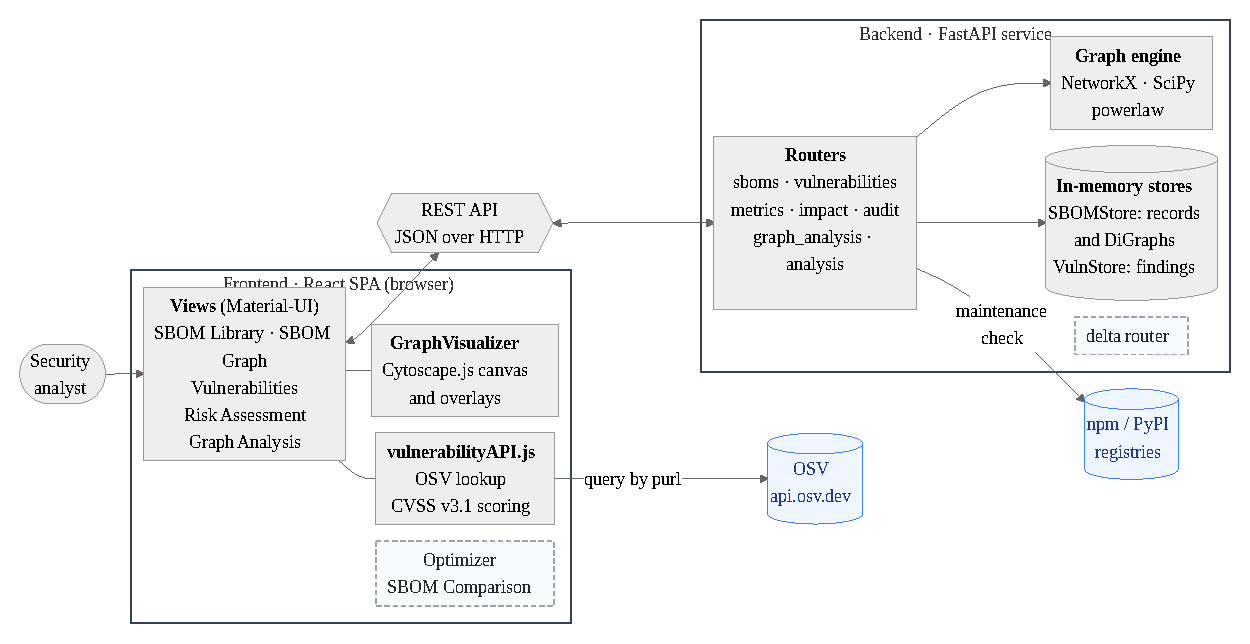
\includegraphics[width=\textwidth]{Figures/Chapter4/architecture.pdf}
%     \caption[SBOM Lens system architecture]{SBOM Lens three-layer architecture. Modules outside the thesis scope (Topology Optimiser, Comparison/Delta) are visually distinguished.}
%     \label{fig:architecture}
% \end{figure}


\subsection{Frontend Layer}
\label{sec:frontend}

The frontend is a React single-page application styled with the Material-UI (MUI) component library. It exposes three primary views: the SBOM Graph (the central visualisation canvas), the Vulnerability Dashboard (aggregated CVE data and remediation status), and the Graph Analysis panel (network-science metric display). A persistent side navigation bar connects the views and hosts the SBOM selection control.

Graph rendering is delegated entirely to Cytoscape.js through a \texttt{GraphVisualizer} React component that holds the Cytoscape instance in a \texttt{useRef} hook. This architectural choice is deliberate: Cytoscape.js manages the HTML5 canvas directly and responds to user gestures with sub-millisecond latency. Routing all canvas operations through React's virtual-DOM reconciler would introduce unnecessary re-render overhead for every pan, zoom, or node drag event. React manages application state --- which SBOM is loaded, which analysis mode is active --- while Cytoscape manages the visual representation.

The data layer is controlled by a compile-time constant \texttt{DATA\_SOURCE} defined in the application configuration file. It switches between \texttt{'localStorage'} (an offline convenience mode used during frontend development) and \texttt{'api'} (the production path that calls the FastAPI backend). The thesis evaluation uses the \texttt{'api'} mode exclusively. The analysis toolbar, which exposes the overlay modes described in \autoref{cp:vuln-analysis} and \autoref{cp:network-sci}, is visible only in API mode when an SBOM is loaded.


\subsection{Backend Layer}
\label{sec:backend}

The backend is a FastAPI application defined in \texttt{main.py} with seven routers registered at startup: \texttt{sboms}, \texttt{vulnerabilities}, \texttt{metrics}, \texttt{impact}, \texttt{audit}, \texttt{graph\_analysis}, and \texttt{delta}. Registration order is significant: the \texttt{delta} and \texttt{graph\_analysis} routers are registered before \texttt{sboms} to prevent FastAPI's wildcard path parameter \texttt{\{sbom\_id\}} from greedily intercepting fixed paths such as \texttt{/sboms/compare}.

The graph engine is NetworkX's \texttt{DiGraph} class. All structural algorithms operate directly on the stored \texttt{DiGraph} object: these include articulation-point detection, k-core decomposition, HITS centrality, Louvain community detection, spectral radius estimation, and the epidemic propagation model, all described in \autoref{cp:network-sci}. This avoids any serialisation step between storage and computation: the router receives a Python object reference, runs the algorithm, and returns results without intermediate conversion.

Several routers maintain per-SBOM result caches at the module level. Community detection and k-core results are expensive to recompute for large graphs; caching ensures that repeated requests for the same SBOM complete in constant time. All caches are explicitly invalidated when an SBOM is updated or deleted, guaranteeing consistency between the stored graph and any cached analytical results.


\subsection{Communication: REST API}
\label{sec:rest-api}

The REST API is served at \texttt{http://localhost:8000} by default, overridable via an environment variable. CORS is configured to permit requests from the React development server. A health endpoint at \texttt{GET /health} returns a JSON object confirming the service status and version number; the frontend uses this to detect backend availability before enabling API-mode features.

The endpoints directly relevant to this chapter are: \texttt{POST /sboms} (file upload, graph construction, and storage), \texttt{GET /sboms/\{id\}} (retrieve a stored SBOM record), and \texttt{GET /sboms/\{id\}/metrics} (returns graph-level metrics including node count, edge count, average out-degree, and the five most-depended-on components ranked by in-degree). The remaining endpoints --- \texttt{/vulnerabilities}, \texttt{/\{id\}/impact}, \texttt{/\{id\}/audit}, \texttt{/\{id\}/graph-analysis}, \texttt{/\{id\}/kcore}, \texttt{/\{id\}/communities}, and \texttt{/\{id\}/epidemic} --- are described in \autoref{cp:vuln-analysis} and \autoref{cp:network-sci} respectively.


\section{CycloneDX Parsing Pipeline}
\label{sec:parsing-pipeline}

Every SBOM in SBOM Lens enters through a single ingest endpoint and exits as a cached \texttt{nx.DiGraph} that all downstream routers query directly. The pipeline is designed for a ``parse once, query many times'' pattern: the graph is built on first ingest and never re-parsed unless the SBOM is explicitly updated. The three subsections trace each stage: upload and duplicate detection, component extraction and node creation, and dependency iteration and edge construction.


\subsection{Ingestion and Deduplication}
\label{sec:ingestion}

SBOM ingestion begins at the \texttt{POST /sboms} endpoint, which accepts a multipart file upload. The raw file bytes are read in full before any graph construction begins, allowing the system to perform two correctness checks upfront.

The first check is JSON validation. The raw bytes are passed to \texttt{json.loads()}; if parsing fails, an HTTP 400 response is returned immediately. This guard ensures that no partially constructed graph can enter the store from a malformed file.

The second check is duplicate detection. A SHA-256 hash of the raw file bytes is computed with \texttt{hashlib.sha256(contents).hexdigest()} and compared against the \texttt{"hash"} field of every stored SBOM record. If a match is found, the endpoint returns \texttt{\{"isDuplicate": True, "existingSBOM": existing\}} without re-storing the file or reconstructing the graph. This ``parse once, query many times'' design avoids redundant computation and prevents double-counting in metrics when the same SBOM is submitted more than once.

A capacity limit prevents unbounded memory growth: the \texttt{MAX\_SBOMS} environment variable (default: 10) caps the number of concurrently stored SBOMs. An upload that would exceed the limit is rejected with HTTP 409 Conflict. This limit is appropriate for a research prototype evaluated on a fixed dataset.


\subsection{Component Extraction}
\label{sec:component-extraction}

Once the file passes validation and deduplication, the CycloneDX JSON structure is traversed to extract components. The root component --- the project or application being described by the SBOM --- is extracted from the \texttt{metadata.component} field and prepended to the \texttt{components[]} list. This placement gives the root a consistent position in the graph and allows the frontend to distinguish it visually as the primary node.

Each entry in the assembled component list is processed into a NetworkX node. The node identifier is resolved through a three-level fallback chain: \texttt{bom-ref} (the CycloneDX primary identifier) is used if present; otherwise \texttt{purl} (Package URL) is used; otherwise the component \texttt{name}. This chain mirrors the CycloneDX field hierarchy defined in \autoref{sec:sbom-cyclonedx} and ensures stable, unique node identifiers across SBOMs produced by different tools with varying levels of metadata completeness.

Node attributes are stored as the NetworkX node's data dictionary. To avoid compatibility issues with NetworkX's attribute handling, only scalar values --- strings, integers, floats, and booleans --- are retained from the component object. In practice, the persisted attributes are \texttt{name}, \texttt{version}, \texttt{purl}, \texttt{type}, and \texttt{bom-ref}. Components for which all three identifier fallbacks yield an empty or \texttt{None} value are silently skipped, making the parser tolerant of incomplete SBOMs encountered in the wild.


\subsection{Graph Construction from Dependencies}
\label{sec:graph-construction}

After all nodes are created, the \texttt{dependencies[]} array is iterated to construct directed edges. Each entry in this array follows the CycloneDX dependency schema: a \texttt{ref} field identifying the depending component, and a \texttt{dependsOn} list identifying the components it depends upon. For each \texttt{(ref, target)} pair, a directed edge is added to the graph with \texttt{G.add\_edge(ref, target)}.

The edge direction encodes a fundamental semantic: an edge from A to B means ``A depends on B''. This directed convention underpins all downstream traversal algorithms. Blast-radius computation, for example, uses \texttt{nx.ancestors(G, node\_id)} to find all components that transitively depend on a given node --- ancestors in the directed graph are precisely those dependants, consistent with the \texttt{ref} \(\to\) \texttt{target} edge direction.

Before adding each edge, a guard verifies that both \texttt{ref} and \texttt{target} already exist as nodes in the graph. Entries in \texttt{dependencies[]} that reference undeclared components are silently skipped. This tolerance is necessary because real-world SBOMs do not always maintain a complete correspondence between the \texttt{components[]} and \texttt{dependencies[]} sections.

The resulting \texttt{nx.DiGraph} is stored in \texttt{SBOMStore.graphs[sbom\_id]} and never re-parsed unless the SBOM is explicitly updated via \texttt{PUT /sboms/\{id\}}. All downstream routers retrieve the graph by calling \texttt{sbom\_store.get\_graph(sbom\_id)}, receiving a direct reference to the live \texttt{DiGraph} object with zero serialisation overhead.


\section{Graph Data Model}
\label{sec:graph-data-model}

The directed graph constructed by the parsing pipeline (\autoref{sec:parsing-pipeline}) encodes the SBOM's component and dependency structure in a form that all downstream algorithms can consume directly. This section defines the node and edge data model --- the representation used by all algorithms in \autoref{cp:vuln-analysis} and \autoref{cp:network-sci}. The in-memory store that manages graph lifecycle is described last.


\subsection{Node Representation}
\label{sec:node-representation}

Each node in the \texttt{DiGraph} represents one software component as declared in the CycloneDX SBOM. The graph contains exactly one node per distinct component identifier, as determined by the \texttt{bom-ref}/\texttt{purl}/\texttt{name} fallback chain described in \autoref{sec:component-extraction}. The node identifier --- the key used to reference the node in all NetworkX operations --- is a stable string assigned at ingest time and unchanged for the lifetime of the stored SBOM.

Each node carries a data dictionary with the following attributes:

\begin{itemize}
    \item \texttt{name} --- human-readable display label for the component.
    \item \texttt{version} --- semantic version string as declared in the SBOM.
    \item \texttt{purl} --- Package URL, used as the primary lookup key when matching components against vulnerability databases in \autoref{cp:vuln-analysis}.
    \item \texttt{type} --- CycloneDX component type; one of \texttt{library}, \texttt{framework}, or \texttt{application}.
    \item \texttt{bom-ref} --- the original CycloneDX \texttt{bom-ref} string, preserved for traceability back to the source file.
\end{itemize}

The root component (extracted from \texttt{metadata.component}) is a regular node in the NetworkX graph. The frontend distinguishes it visually by setting an \texttt{isPrimary} flag in the Cytoscape node data object produced by \texttt{convertCycloneDXToGraph()}, which triggers a distinct green fill on the canvas.


\subsection{Edge Representation}
\label{sec:edge-representation}

Each directed edge represents a direct dependency relationship between two components. An edge from node A to node B encodes the statement: \textit{A directly depends on B}. This follows from the CycloneDX dependency schema, where an entry \texttt{(ref: A, dependsOn: [B, ...])} produces the directed edge A \(\to\) B.

This directed semantics is load-bearing for every traversal algorithm in the system. Blast-radius analysis identifies all components that would be affected if a given component were compromised; these are its \textit{ancestors} in the directed graph --- the nodes from which there exists a directed path to the target, consistent with the A \(\to\) B convention. Dominator-tree construction, depth histograms, and topological ordering all depend on the same directed convention, as described in \autoref{cp:vuln-analysis} and \autoref{cp:network-sci}.

No attributes are stored on NetworkX edges. Edges are pure structural connectors: their presence encodes a dependency, and their direction encodes which component depends on which. On the frontend, each Cytoscape edge object carries an identifier formed from the source and target node IDs, a static label \texttt{depends\_on}, and the CSS class \texttt{default-edge} for baseline styling.


\subsection{In-Memory Store}
\label{sec:in-memory-store}

The \texttt{SBOMStore} class manages the lifecycle of all stored SBOMs and their corresponding graphs. It maintains two parallel dictionaries: \texttt{self.sboms} maps each SBOM identifier to a full record dictionary (containing the SHA-256 hash, display name, creation timestamp, and the raw CycloneDX component and dependency lists); \texttt{self.graphs} maps the same identifier to the corresponding \texttt{nx.DiGraph}.

When a router needs to perform graph analysis, it retrieves the stored \texttt{DiGraph} via the store's \texttt{get\_graph} method, which returns a direct Python reference to the live object. There is no serialisation step between storage and computation: the algorithm receives the graph object and operates on it in place. This design minimises latency for interactive analysis queries, where sub-second response times are necessary for a usable graph exploration interface.

Several routers maintain module-level caches for computationally expensive results --- community detection and k-core decomposition are cached after the first request for a given SBOM. These caches are explicitly invalidated whenever an SBOM is updated or deleted, ensuring that stale results are never returned to the frontend.

As noted in \autoref{sec:architecture-overview}, the store's state is ephemeral: a server restart clears all SBOMs and graphs. This design is appropriate for the research context, and persistent storage is listed as a limitation and direction for future work in \autoref{cp:conclusion}.


\section{SBOM Graph Visualisation}
\label{sec:graph-visualisation}

The SBOM Graph is the primary interface through which the user explores the dependency structure of a loaded SBOM. This section describes the base rendering layer implemented with Cytoscape.js, the three available layout algorithms, and the core interaction model. Analysis overlays --- vulnerability highlighting (\autoref{cp:vuln-analysis}) and network-science colouring (\autoref{cp:network-sci}) --- extend the base layer described here.


\subsection{Graph Rendering with Cytoscape.js}
\label{sec:cytoscape-rendering}

Cytoscape.js is initialised imperatively inside the \texttt{GraphVisualizer} React component using the \texttt{useRef} and \texttt{useEffect} hooks. The Cytoscape instance is stored in a ref rather than component state, so operations on the canvas --- panning, zooming, applying a new layout --- do not trigger React's reconciliation cycle. This separation keeps the graph canvas responsive under interactive load.

The default visual encoding uses a consistent style throughout the application. Component nodes are rendered as circular shapes (\(28 \times 28\) pixels) filled with Material-UI's info blue, with the component name displayed as a label below the node. The root component --- the project whose dependencies are being analysed --- is distinguished by a green fill and a 2-pixel border, making it immediately identifiable as the anchor of the dependency tree. Dependency edges are rendered as Bézier curves with triangle arrowheads at the target end, indicating the direction of dependency. Edges carry the static label \texttt{depends\_on} with auto-rotate enabled so the label follows the curve.

Overlay CSS classes are pre-defined in the Cytoscape stylesheet and applied programmatically when an analysis mode is activated. The pre-defined overlay classes are: \texttt{.articulation-point} (red), \texttt{.blast-radius} (purple), \texttt{.dominator-tree} (cyan), \texttt{.vuln-node} (orange), \texttt{.diamond-node} (green), and \texttt{.hits-active} (node size and colour scaled from HITS score attributes). A \texttt{.dimmed} class reduces opacity to 15\,\% to grey out nodes and edges that are not part of the current selection or overlay. The analytical meaning of each overlay class is defined in \autoref{cp:vuln-analysis} and \autoref{cp:network-sci}; this section establishes the visual layer only.


\subsection{Layout Algorithms}
\label{sec:layouts}

SBOM Lens exposes three Cytoscape.js layout algorithms, accessible via toolbar buttons, each suited to a different graph exploration objective.

The \textbf{Tree Layout} (Cytoscape name: \texttt{breadthfirst}, \texttt{directed: true}) organises nodes in horizontal levels according to their distance from the root in a breadth-first traversal. This layout makes dependency depth immediately visible: direct dependencies appear on level one, transitive dependencies on level two and beyond. It is the default layout for the Delta and Comparison views, where structural differences between two SBOMs are easier to compare when both graphs share the same hierarchical orientation.

The \textbf{Radial Layout} (Cytoscape name: \texttt{concentric}) places nodes in concentric rings around a central hub, with the root component at the centre. This is the default layout applied when a new SBOM is first loaded, giving the user an immediate overview of the dependency neighbourhood around the root.

The \textbf{Force-Directed Layout} (Cytoscape name: \texttt{cose}) simulates a physical spring system to distribute nodes so that connected components cluster together organically without imposing a hierarchical structure. This layout is particularly effective for revealing natural groupings in large, densely connected SBOMs.

All three layouts share common configuration options: \texttt{fit: true} (zoom to fit the graph on screen), a padding of 150 pixels, overlap avoidance, and an animated transition of 600\,ms. Layout changes are applied imperatively by re-running the Cytoscape algorithm on the existing node and edge data without issuing a new request to the backend.


\subsection{Core Interaction Model}
\label{sec:interaction-model}

The SBOM Graph supports the following core interactions, designed to enable focused exploration of the dependency structure.

\textbf{Node selection.} Tapping a node selects it; a blue border is applied to the highlighted node. Tapping the canvas background deselects all nodes.

\textbf{Node inspection.} Selecting a node opens a sidebar panel displaying the node's stored attributes: \texttt{name}, \texttt{version}, \texttt{purl}, \texttt{type}, and \texttt{bom-ref}. This panel gives the analyst the metadata needed to cross-reference the selected component with external vulnerability databases.

\textbf{Zoom and fit.} The current zoom level is tracked in React component state and displayed in the toolbar. A fit-to-view button resets the viewport so the entire graph is visible, which is useful after navigating to a deeply nested subgraph.

\textbf{SBOM selection.} A selector component lists all SBOMs currently stored in \texttt{SBOMStore}. Selecting an SBOM converts the stored CycloneDX data to Cytoscape node and edge objects and loads them into the Cytoscape instance.

\textbf{Impact analysis entry point.} Right-clicking a node opens a context menu that includes an impact analysis option, which fetches blast-radius and dominator-tree data from the backend. The analytical meaning of the resulting overlay is described in \autoref{cp:vuln-analysis}; the interaction gesture is documented here as part of the interaction model.

Dynamic graph editing features --- adding new nodes, repositioning nodes by dragging, and creating edges via the \texttt{cytoscape-edgehandles} plugin --- are implemented in the application but are outside the scope of this thesis. These are graph construction utilities, not structural risk assessment features, and are not evaluated in this work.

\chapter[Vulnerability Analysis]{Vulnerability Analysis}
\label{cp:vuln-analysis}

\autoref{cp:system-design} established the directed dependency graph that SBOM Lens constructs from a CycloneDX SBOM. Every node in that graph carries a \texttt{purl} attribute --- a Package URL uniquely identifying the component --- as defined in \autoref{sec:node-representation}. \autoref{cp:vuln-analysis} uses those PURL attributes as the anchor for vulnerability matching: by querying the Open Source Vulnerabilities database (OSV) with the PURLs present in the graph, SBOM Lens enriches the structural model with real-world risk data. OSV aggregates advisories from the GitHub Advisory Database, the PyPA advisory database and many other upstream sources, so a single PURL-native query reaches all of them. The chapter is organised into five sections. \autoref{sec:multi-source} describes why OSV is the vulnerability source and how the integration pipeline works. \autoref{sec:dedup-storage} describes how vulnerability records are stored in the in-memory \texttt{VulnStore} and deduplicated by CVE ID and PURL pair. \autoref{sec:cvss-computation} explains how CVSS v3.1 base scores are computed on the client side and maps scores to the severity bands used throughout the system. \autoref{sec:vuln-workflow} covers the analyst-facing management workflow: automated fetching on SBOM upload and the three-state status lifecycle exposed through the REST API. \autoref{sec:graph-overlay} describes how vulnerability data is projected back onto the Cytoscape graph as three distinct overlay types --- severity colour coding, blast-radius highlighting, and dominator-tree highlighting --- giving analytical meaning to the CSS overlay classes introduced in \autoref{sec:cytoscape-rendering}.


\section{Vulnerability Source}
\label{sec:multi-source}

Matching SBOM components against known vulnerabilities requires querying an external database that maintains curated records of published vulnerabilities. This section justifies the choice of OSV as that database and describes the integration pipeline.


\subsection{Rationale for OSV}
\label{sec:multi-source-rationale}

No single vulnerability database covers all software ecosystems with equal completeness, and databases differ in how precisely they identify the affected package. NVD, maintained by NIST, identifies products with Common Platform Enumeration (CPE) strings, a scheme designed for commercial software. As noted in \autoref{sec:cve-nvd}, matching open-source packages against CPE strings is imprecise: a package may have several CPE strings or none, and name-based matching can return vulnerabilities for unrelated products that share a name. OSV, by contrast, was designed from the outset to accept PURL queries and to express affected versions as ranges, which makes it precise for exactly the identifiers an SBOM carries.

OSV is also an aggregator. It ingests the GitHub Advisory Database (GHSA), the PyPA advisory database, RustSec, the Go vulnerability database, and many other upstream sources, and each entry cross-references CVE and GHSA identifiers in its \texttt{aliases} field \citep{OSV}. A single OSV query therefore reaches the advisory data that separate GHSA or NVD queries would have provided for open-source packages, without the imprecise name-to-product mapping that NVD requires. Finally, OSV requires no API key, so SBOM Lens produces vulnerability results in any environment without prior registration.

SBOM Lens therefore uses OSV as its sole vulnerability source. The cost of this choice is dependence on OSV's aggregation: an advisory published upstream reaches SBOM Lens only once OSV has ingested it, and vulnerabilities that exist only in NVD, without an open-source advisory, are not reported. Direct integration of further sources is discussed as future work in \autoref{cp:conclusion}.


\subsection{OSV Integration Pipeline}
\label{sec:osv-pipeline}

The OSV integration is implemented as a two-phase pipeline in \texttt{fetchVulnerabilitiesForSBOM()} inside \texttt{vulnerabilityAPI.js}. The first phase issues a single batch request to the \texttt{/v1/querybatch} endpoint with an array of PURL queries --- one entry per component in the loaded SBOM. This batch design avoids \(N\) serial HTTP requests for an SBOM with \(N\) components: the entire component list is submitted in one round-trip, and the response returns the matching OSV vulnerability IDs for each PURL position.

The second phase resolves each unique OSV ID to its full advisory record by fetching \texttt{/v1/vulns/\{id\}}. The detail record contains the canonical summary, published and modified dates, a list of CVSS severity objects, and an \texttt{aliases} array that may include CVE identifiers. CVE alias resolution is performed by scanning the \texttt{aliases} array for an entry beginning with the prefix \texttt{"CVE-"}: the first such alias becomes the canonical \texttt{cveId} stored in \texttt{VulnStore}. If no CVE alias is present, the OSV identifier itself is used as the \texttt{cveId} fallback; deduplication logic (\autoref{sec:dedup-logic}) still operates correctly on OSV IDs.

Severity is derived in three steps. If the \texttt{severity[]} array of the detail record contains an entry whose \texttt{type} is \texttt{"CVSS\_V3"}, its \texttt{score} field --- a CVSS vector string rather than a pre-computed number --- is passed to \texttt{cvssV3BaseScore()} (\autoref{sec:cvss-implementation}) and the resulting base score is mapped to a severity band. CVSS v4 vectors are not scored, because the v3.1 formula does not apply to them. If no v3 vector is present, the severity label that the originating advisory database attaches to the record (\texttt{database\_specific.severity}, as published by GHSA) is used, with GHSA's \textsc{moderate} mapped to \textsc{medium}. If neither is available, the record's severity is \textsc{unknown}; it is never silently treated as \textsc{low}.

The pipeline is invoked automatically through the \texttt{useVulnerabilityFetcher} React hook whenever an SBOM is uploaded to the library. The hook follows a fire-and-forget pattern: it is asynchronous, no error is ever shown to the analyst, and the graph view is never blocked waiting for vulnerability data to arrive. Records are injected into \texttt{VulnStore} sequentially rather than in parallel: submitting all records in parallel would cause duplicate POSTs to race the backend deduplication check before it has processed the first record. When an upload contains pairs already in the store --- because another SBOM shares the component, or because the same SBOM is uploaded again after being deleted --- the backend rejects each with HTTP 409, and the frontend hook treats 409 as a no-op, so the analyst observes no duplication.


\section{Deduplication and Storage}
\label{sec:dedup-storage}

The same vulnerability can reach the store more than once: the fetch runs for every SBOM uploaded, and SBOMs in one library often share components; and an analyst can also enter records manually. \texttt{VulnStore} is the in-memory store that absorbs these records and ensures that each unique vulnerability-component pair is stored exactly once. This section describes the storage schema and the deduplication logic.


\subsection{VulnStore Design}
\label{sec:vulnstore-design}

\texttt{VulnStore} is implemented as a Python class in \texttt{backend/store/vuln\_store.py}. It maintains a single in-memory dictionary, \texttt{self.vulns}, keyed by UUID strings generated at record creation time with \texttt{str(uuid.uuid4())}. State is ephemeral: the dictionary is cleared on server restart, consistent with the ephemeral design of \texttt{SBOMStore} described in \autoref{sec:in-memory-store} and appropriate for a research prototype evaluated on a fixed dataset.

Each record in \texttt{self.vulns} conforms to a consistent schema:

\begin{itemize}
    \item \textbf{id} --- UUID string uniquely identifying the record.
    \item \textbf{purl} --- Package URL of the affected component, matching the node attribute described in \autoref{sec:node-representation}.
    \item \textbf{cveId} --- CVE identifier or OSV identifier if no CVE alias was resolved.
    \item \textbf{severity} --- severity band (\textsc{critical}, \textsc{high}, \textsc{medium}, \textsc{low}, or \textsc{unknown}) derived as described in \autoref{sec:osv-pipeline}.
    \item \textbf{status} --- current remediation status; one of \texttt{NOT\_STARTED}, \texttt{IN\_PROGRESS}, or \texttt{REMEDIATED}.
    \item \textbf{patchAvailable} --- boolean, set by the analyst when entering a record manually, indicating that a patched version is known to exist; records from the OSV fetch always carry \texttt{false}.
    \item \textbf{notes} --- free-text analyst annotation.
    \item \textbf{source} --- origin of the record: \texttt{"osv"} for the automatic fetch or \texttt{"Manual"} for analyst entry.
    \item \textbf{publishedDate} --- date the advisory was first published.
    \item \textbf{lastUpdated} --- server-side timestamp refreshed on each \texttt{PUT} update.
    \item \textbf{timeline} --- list of status-transition objects, each carrying a timestamp, the new status value and a note, recording the remediation history of the record.
\end{itemize}

The \texttt{source} field preserves the provenance of each record, allowing an analyst to distinguish vulnerabilities found by the automatic OSV scan from those entered manually.


\subsection{Deduplication Logic}
\label{sec:dedup-logic}

Deduplication is enforced in the \texttt{VulnStore.add()} method before any new record is committed to the store. The dedup key is the pair of \texttt{cveId} and \texttt{purl}: the method searches the existing records for any entry where both fields match the incoming record.

\begin{verbatim}
duplicate = next((v for v in self.vulns.values()
    if v.get("cveId") == cve_id and v.get("purl") == purl), None)
\end{verbatim}

If a matching record is found, \texttt{add()} returns \texttt{None} without modifying the store. The REST endpoint wrapping this method responds with HTTP 409 Conflict. The \texttt{useVulnerabilityFetcher} hook treats a 409 response as a silent no-op: no error is raised, no duplicate appears in the store, and the analyst sees no change.

OSV IDs that could not be resolved to a CVE alias retain their OSV identifier as the \texttt{cveId} field; the deduplication logic operates on that OSV ID equally well, preventing duplicates when the same OSV entry is fetched again for another SBOM. Because the key is the first CVE alias, two distinct advisories that share that alias for the same component are also collapsed into one record, and the advisory stored second is discarded.

The first-written record for a pair is kept: a later record for the same pair, for example a manual entry with a different severity, is rejected rather than merged.


\section{CVSS v3.1 Base Score Computation}
\label{sec:cvss-computation}

Vulnerability records from the OSV pipeline carry CVSS vector strings rather than pre-computed numeric scores. SBOM Lens computes base scores from these vectors entirely on the client side, with no dependency on an external CVSS scoring service. This section describes how the CVSS v3.1 formula is applied, illustrates the computation with the Log4Shell vector, and explains the design of the custom JavaScript implementation.


\subsection{Formula and Metric Groups}
\label{sec:cvss-formula}

The CVSS v3.1 base score formula and the numerical values for each metric are fully defined in \autoref{sec:cvss}; this section does not repeat that derivation, but states explicitly the severity band thresholds that SBOM Lens uses to map numeric scores to visual encodings.

SBOM Lens maps CVSS base scores to four severity bands, plus \textsc{unknown} for records without any usable severity (\autoref{sec:osv-pipeline}):

\begin{center}
    \begin{tabular}{ll}
        \toprule
        \textbf{Severity} & \textbf{Score Range} \\
        \midrule
        \textsc{critical} & \(\geq 9.0\) \\
        \textsc{high} & \(7.0\)--\(8.9\) \\
        \textsc{medium} & \(4.0\)--\(6.9\) \\
        \textsc{low} & \(< 4.0\) \\
        \bottomrule
    \end{tabular}
\end{center}

These thresholds follow the NVD/NIST severity rating scale. FIRST.org's published five-band scheme adds a ``None'' band for a base score of exactly \(0.0\); SBOM Lens collapses this band into \textsc{low} to simplify the overlay colour mapping to four distinct visual classes. When the input to \texttt{parseCVSSSeverity()} is missing or cannot be scored, the function returns \textsc{unknown} rather than defaulting to \textsc{low}, so that missing severity data is not mistaken for low risk. On the graph, \textsc{unknown} nodes are drawn with the \textsc{low} colour; in the data, and in the evaluation of \autoref{cp:evaluation}, they remain a separate band.

The scope-sensitivity of the Privileges Required (PR) metric is handled explicitly: when Scope is Changed (\texttt{S:C}), the PR Low coefficient is \(0.68\) rather than \(0.62\), and the PR High coefficient is \(0.50\) rather than \(0.27\); PR None is \(0.85\) in both cases. The custom implementation branches on the parsed Scope value when looking up PR coefficients, matching the FIRST.org specification precisely.


\subsection{Worked Example: Log4Shell}
\label{sec:cvss-log4shell}

Log4Shell (\texttt{CVE-2021-44228}) was introduced as the principal illustrative case study in \autoref{sec:cvss} and analysed from a supply-chain perspective in \autoref{sec:case-log4shell}. \autoref{cp:vuln-analysis} applies the same vulnerability to the implementation: given its CVSS vector, the client-side scoring function must produce the expected base score.

The Log4Shell vector is:
\begin{center}
    \texttt{CVSS:3.1/AV:N/AC:L/PR:N/UI:N/S:C/C:H/I:H/A:H}
\end{center}

Substituting the numerical values specified in \autoref{sec:cvss} gives: \(AV = 0.85\), \(AC = 0.77\), \(PR = 0.85\) (Scope Changed branch), \(UI = 0.85\), \(C = 0.56\), \(I = 0.56\), \(A = 0.56\). The Impact Sub-Score (ISS) is:
\[
    \mathit{ISS} = 1 - (1 - 0.56)(1 - 0.56)(1 - 0.56) = 1 - 0.44^3 = 1 - 0.0852 \approx 0.9148
\]

Because Scope is Changed, the Impact term uses the modified formula:
\begin{align*}
    \mathit{Impact} &= 7.52 \times (\mathit{ISS} - 0.029) - 3.25 \times (\mathit{ISS} - 0.02)^{15} \\
    &\approx 7.52 \times 0.8858 - 3.25 \times 0.8948^{15} \\
    &\approx 6.661 - 0.614 \approx 6.048
\end{align*}

The Exploitability term is:
\[
    \mathit{Exploitability} = 8.22 \times 0.85 \times 0.77 \times 0.85 \times 0.85 \approx 3.887
\]

The base score is therefore:
\begin{align*}
    \mathit{Base} &= \min\bigl(1.08 \times (6.048 + 3.887),\ 10\bigr) \\
    &= \min(1.08 \times 9.935,\ 10) \\
    &= \min(10.73,\ 10) = 10.0
\end{align*}

The CVSS roundup rule produces a final score of \(10.0\), which falls in the \textsc{critical} band (\(\geq 9.0\)). In the graph overlay described in \autoref{sec:severity-colour}, a Log4Shell-affected component node is therefore assigned the \texttt{.vuln-critical} CSS class and rendered in red.


\subsection{Custom Client-Side Implementation}
\label{sec:cvss-implementation}

The CVSS scoring logic is implemented entirely in \texttt{vulnerabilityAPI.js} with no external CVSS library dependency. This is a deliberate design choice: adding a CVSS computation library to the frontend \texttt{package.json} would introduce a runtime dependency whose licensing, maintenance status, and specification compliance would need independent verification. Implementing the formula from the FIRST.org specification in approximately seventy lines of JavaScript keeps the frontend self-contained and makes the scoring logic directly auditable alongside the rest of the source code.

The function \texttt{cvssV3BaseScore(vector)} accepts a CVSS vector string, splits it on the \texttt{"/"} separator to extract metric abbreviation--value pairs, and looks each pair up in a coefficient table to produce the numeric values used in the formulas above. It branches on the parsed Scope value to select the correct Impact and PR coefficients, computes the ISS, Impact, Exploitability, and Base sub-terms in sequence, and applies the CVSS roundup rule (\texttt{Math.ceil(base * 10) / 10}) before returning the final score. This roundup rule is specified by FIRST.org as ``the smallest number, specified to one decimal place, that is equal to or higher than its input''; the expression \texttt{Math.ceil(x * 10) / 10} implements it exactly.

The entry point for callers is \texttt{parseCVSSSeverity(scoreString)}, which accepts either a numeric score string (e.g.\ \texttt{"9.8"}) or a CVSS v3 vector string (as returned by OSV). If the input does not parse as a number and begins with \texttt{"CVSS:"}, it is treated as a vector and passed to \texttt{cvssV3BaseScore()}. This single entry point means the rest of the codebase does not need to distinguish numeric scores from vectors.


\section{Vulnerability Management Workflow}
\label{sec:vuln-workflow}

Beyond recording which components carry known CVEs, SBOM Lens provides a lightweight remediation-tracking workflow. Analysts can update the status of each vulnerability record, add notes, and observe how the record's status has changed over time. This section describes the automated fetch that populates the store on SBOM upload and the REST API that exposes the status lifecycle.


\subsection{Automated Fetch on SBOM Upload}
\label{sec:automated-fetch}

Vulnerability fetching is triggered automatically when an SBOM is uploaded to the library, without requiring any analyst action. The \texttt{useVulnerabilityFetcher} React hook receives the \texttt{components[]} array from the uploaded SBOM and passes the PURL list to the OSV pipeline described in \autoref{sec:osv-pipeline}.

The hook follows the fire-and-forget pattern introduced in \autoref{sec:osv-pipeline}: it is asynchronous, does not block rendering, and never surfaces an error to the analyst: a failed OSV request yields an empty result, and a backend error while storing records is logged with \texttt{console.warn} and abandons the remaining records of that SBOM. A network failure therefore never prevents the analyst from viewing the dependency graph, but an empty vulnerability list cannot be told apart from a failed lookup. Records are submitted to the backend's \texttt{POST /vulnerabilities} endpoint one at a time rather than in a batch request; this sequential submission prevents a parallel flood of identical records from racing the deduplication check on the server side.

Because records are keyed by CVE ID and PURL rather than by SBOM, an upload that shares components with an SBOM already in the library resubmits pairs that already exist in \texttt{VulnStore}; so does an SBOM uploaded again after being deleted, since deleting an SBOM does not delete its vulnerability records. Each such pair receives a 409 Conflict response, which the hook treats as a no-op. Vulnerabilities are fetched once, at upload: selecting an SBOM or reloading the page does not query OSV again, so an advisory published later reaches an SBOM only if it is uploaded again.


\subsection{Status Lifecycle and REST API}
\label{sec:status-lifecycle}

\texttt{VulnStore} exposes a full CRUD REST API through the \texttt{vulnerabilities} FastAPI router. The endpoints are:

\begin{itemize}
    \item \texttt{GET /vulnerabilities} --- returns all records in the store as a JSON array; no SBOM-scoping filter is applied, making the store a global view of all known vulnerabilities across all loaded SBOMs.
    \item \texttt{POST /vulnerabilities} --- creates a new record; returns HTTP 201 on success or HTTP 409 if the CVE ID + PURL pair already exists.
    \item \texttt{PUT /vulnerabilities/\{id\}} --- partial update of an existing record: every field sent replaces the stored value; the interface uses it to change \texttt{status} and extend \texttt{timeline}. The \texttt{lastUpdated} timestamp is set by the server.
    \item \texttt{DELETE /vulnerabilities/\{id\}} --- removes a single record.
    \item \texttt{DELETE /vulnerabilities} --- clears the entire store; useful for resetting state between evaluation runs without restarting the server.
\end{itemize}

The \texttt{status} field supports a three-state remediation lifecycle. \texttt{NOT\_STARTED} is the initial state assigned to every newly created record. \texttt{IN\_PROGRESS} indicates that a remediation effort is under way. \texttt{REMEDIATED} is the terminal state, indicating that the vulnerability has been patched or mitigated. The backend stores the field without validating it, so triage states such as a deliberate decision not to fix, or a false positive, could be added to the interface without changing the API; the evaluated version does not offer them. The first \texttt{timeline} entry is written by the server when the record is created; each later status change made through the interface appends an entry with a client-side timestamp and sends the extended list back. The server does not enforce this, since \texttt{PUT} replaces any field it receives, so the timeline is a remediation history for a single-user prototype rather than a tamper-proof audit trail. \autoref{fig:vulnerabilities-page} shows the Vulnerabilities page, where the analyst reviews the stored records and changes their status.

\begin{figure}[!htpb]
    \centering
    \screenshot{Figures/Chapter5/vulnerabilities-page}{Vulnerabilities page with the \texttt{code-server} SBOM selected: severity totals and the records table, with the Component column now filled in. Light theme, same window size as the other screenshots.}
    \caption[The Vulnerabilities page]{The Vulnerabilities page for the \texttt{code-server} SBOM: totals by severity band, and the stored vulnerability records with their component, severity band and remediation status.}
    \label{fig:vulnerabilities-page}
\end{figure}


\section{Graph Overlay Visualisation}
\label{sec:graph-overlay}

The vulnerability data held in \texttt{VulnStore} is projected back onto the Cytoscape.js graph through three distinct overlay types. Each overlay assigns one of the CSS classes pre-defined in \autoref{sec:cytoscape-rendering} --- \texttt{.vuln-critical}, \texttt{.vuln-high}, \texttt{.vuln-medium}, \texttt{.vuln-low}, \texttt{.blast-radius}, and \texttt{.dominator-tree} --- to the appropriate nodes, giving those classes the analytical meaning that \autoref{cp:system-design} deferred to this chapter. All three overlays are activated interactively by the analyst: the severity colour-coding overlay from the Analysis menu, and the blast-radius and dominator-tree overlays from the same menu, for the node chosen with \emph{Analyze Impact} in its context menu.


\subsection{Severity Colour Coding}
\label{sec:severity-colour}

The severity colour-coding overlay is activated from the Analysis menu once vulnerability records for the loaded SBOM are present in \texttt{VulnStore}. When it is active, each graph node is assigned a CSS overlay class determined by the highest-severity CVE that affects the component identified by that node's PURL.

A component may carry multiple CVE records in \texttt{VulnStore}; in that case the highest severity wins. A node whose PURL is associated with one \textsc{critical} and three \textsc{medium} vulnerabilities is displayed as \textsc{critical} --- the most dangerous exposure takes visual precedence. The Cytoscape overlay is applied programmatically: for each node, the vulnerability records whose \texttt{purl} field matches the node's PURL are retrieved from the store, the maximum of their severity bands (assigned by \texttt{parseCVSSSeverity()} when the records were fetched) is taken, and the node is assigned the matching class (\texttt{.vuln-critical}, \texttt{.vuln-high}, \texttt{.vuln-medium}, or \texttt{.vuln-low}). Nodes whose PURL matches no stored vulnerability record receive no severity class and keep their default colour. \autoref{fig:node-details} in \autoref{cp:system-design} shows the overlay applied to the \texttt{code-server} SBOM, with \texttt{basic-ftp}, its \textsc{critical} component, selected.



\subsection{Blast Radius Analysis}
\label{sec:blast-radius}

The blast-radius overlay is an interactive analysis triggered when the analyst chooses a node with \emph{Analyze Impact} in its context menu and switches the overlay on in the Analysis menu, as described in \autoref{sec:interaction-model}. The query is issued to \texttt{GET /\{sbom\_id\}/impact?node\_id=\{id\}}, which returns the blast radius, dependency paths, dominated nodes, and the HITS hub and authority scores of the queried node in a single response.

On the backend, the blast radius is computed as \texttt{list(nx.ancestors(G, node\_id)) + [node\_id]}. The semantic interpretation follows directly from the edge direction established in \autoref{sec:edge-representation}: an edge from A to B means A depends on B, so \texttt{nx.ancestors(G, B)} returns all nodes from which there exists a directed path to B --- the upstream consumers of B whose security posture is degraded if B is compromised; the blast radius is B together with these consumers. This framing is intentional and distinct from a ``downstream'' interpretation: in the SBOM Lens graph, the upstream consumers are the packages that pull in the vulnerable component, and so the packages that may be affected if the vulnerable node is compromised. Because the analysis is at component level, this over-approximates exposure: a consumer may never execute the vulnerable code (\autoref{sec:rw-call-graphs}).

The API response also includes up to five shortest paths from the root packages (components with in-degree zero) to the vulnerable node, computed with \texttt{nx.all\_shortest\_paths} from each root. These paths provide concrete dependency chains --- a sequence of ``package X uses package Y which uses the vulnerable package Z'' --- that an analyst can use to understand exactly how the vulnerable component entered the dependency tree. The interface lists them in the \emph{Dependency paths} section of the Details panel, together with the total number of paths from the root to the node and the number of consumers they pass through; selecting a path highlights it on the graph, and \emph{Highlight all paths} highlights every edge of the blast radius.

On the frontend, blast-radius nodes receive the \texttt{.blast-radius} CSS class (purple, as pre-defined in \autoref{sec:cytoscape-rendering}). \autoref{fig:blast-radius} shows the overlay for \texttt{basic-ftp}~5.0.3, the component with a \textsc{critical} advisory (CVE-2026-27699) in the \texttt{code-server} SBOM.

\begin{figure}[!htpb]
    \centering
    \screenshot[0.8\textwidth]{Figures/Chapter5/blast-radius}{SBOM Graph page, \texttt{code-server} SBOM: \emph{Analyze Impact} on \texttt{basic-ftp}, Blast Radius and severity overlays active, all paths highlighted. Light theme, same window size as the other screenshots.}
    \caption[Blast-radius overlay]{Blast radius of \texttt{basic-ftp} in the \texttt{code-server} SBOM. Its four consumers --- \texttt{get-uri}, \texttt{pac-proxy-agent}, \texttt{proxy-agent} and the application \texttt{code-server} --- are purple, \texttt{basic-ftp} keeps the red of its \textsc{critical} band, and the edges of the single dependency path are highlighted in orange. The Details panel lists the path, \texttt{code-server} \(\to\) \texttt{proxy-agent} \(\to\) \texttt{pac-proxy-agent} \(\to\) \texttt{get-uri} \(\to\) \texttt{basic-ftp}.}
    \label{fig:blast-radius}
\end{figure}

The impact API response also includes \texttt{hitsHub} and \texttt{hitsAuthority} scores of the analysed component; scores for every node are returned by \texttt{GET /sboms/\{id\}/global-analysis}. These scores quantify the component's structural centrality in the dependency network and are relevant to prioritising remediation effort; however, the HITS algorithm that produces them is described in detail in \autoref{cp:network-sci} (specifically \autoref{sec:hits}) and is not explained further here.


\subsection{Dominator Tree Analysis}
\label{sec:dominator-tree}

The dominator-tree overlay is returned in the same \texttt{GET /\{sbom\_id\}/impact} response as the blast radius, adding structural risk information without requiring an additional round-trip.

On the backend, dominance is computed from the root of the dependency graph, not from the vulnerable node. \texttt{nx.immediate\_dominators(G, root)} returns, for every component reachable from the root, its immediate dominator; when the SBOM has several root components, they are first joined under a virtual root so that a single dominator tree exists. The dominated set of the vulnerable node is then its entire subtree in that dominator tree: every component for which each path from the root passes through the vulnerable node. In supply-chain terms, a node with a non-empty dominated set is a structural chokepoint: if it were removed or replaced, all the dominated components would lose their connection to the application with no alternative route.

Dominated nodes are assigned the \texttt{.dominator-tree} CSS class on the frontend, displayed in cyan as pre-defined in \autoref{sec:cytoscape-rendering}. When both overlays are switched on for the same node, the analyst can read them together: nodes highlighted in purple are the upstream consumers affected by the vulnerability's propagation, while nodes highlighted in cyan are structurally dependent on the vulnerable node and would be isolated if it were removed. This dual encoding gives both a security-propagation view and an architectural-risk view in a single inspection, providing complementary information that neither overlay conveys alone. In the evaluated version, choosing a new node while both overlays are active refreshes only the blast radius, so the dominator-tree overlay must be switched off and on again to follow the new node. \autoref{fig:dominated-set} shows the dominated set of \texttt{express} in the \texttt{code-server} SBOM.

\begin{figure}[!htpb]
    \centering
    \screenshot[0.8\textwidth]{Figures/Chapter5/dominated-set}{SBOM Graph page, \texttt{code-server} SBOM: \emph{Analyze Impact} on \texttt{express}, Dominator Tree and severity overlays active. Light theme, same window size as the other screenshots.}
    \caption[Dominated set]{Dominated set of \texttt{express} in the \texttt{code-server} SBOM (cyan): the components reachable from the root only through \texttt{express}, which would lose their connection to the application if it were removed. The severity colours of the vulnerable components are also shown.}
    \label{fig:dominated-set}
\end{figure}

\chapter[Structural Risk and Graph Analysis]{Structural Risk and Graph Analysis}
\label{cp:network-sci}

% TODO: chapter not yet written. Decisions: docs/adr/0001; vocabulary: CONTEXT.md.
% Central claim: a component's position in the dependency graph carries risk information that
%   flat-inventory analysis cannot express; graph measures make it visible at three scales.
% Organise by scale, not by algorithm:
%   Component scale  -- articulation points and bridges, HITS hub/authority, spectral exposure score
%                       (eigenvector centrality; never "R0"), k-core number; one paragraph on the
%                       optimizer's edge rankings as an application of the spectral score.
%   Cluster scale    -- Louvain communities, bow-tie decomposition, rich-club.
%   Whole-graph scale-- spectral radius and epidemic threshold 1/lambda_1, degree entropy, cycles/SCCs,
%                       version conflicts (not "diamonds"), namespace concentration, power-law fit,
%                       small-world (C, L). Define briefly here; values are reported in Chapter 7 (RQ1).
% Out: blast radius and dominated sets (Chapter 5, refer back); unmaintained check (short note in
%   Chapter 5); WL fingerprinting / SBOM comparison (left out of the thesis); propagation simulation
%   (future work).

\section{Component Scale}
\label{sec:component-scale}

\subsection{HITS Hub and Authority Scores}
\label{sec:hits}

\section{Cluster Scale}
\label{sec:cluster-scale}

\section{Whole-Graph Scale}
\label{sec:structural-risk}

\chapter[Evaluation]{Evaluation}
\label{cp:evaluation}

% TODO: chapter not yet written. Promised by Chapters 1-2: real-world open-source SBOM dataset;
%   graph-level metrics (degree distribution / power law, clustering coefficient, average path length);
%   node-level metrics; vulnerability findings; structural analysis results; discussion.

\chapter[Conclusion]{Conclusion}
\label{cp:conclusion}

% TODO: chapter not yet written. Everything except the summary of findings can be written now.
% Contributions: map one-to-one to RO1-RO4 (Section 1.3).
% Limitations: in-memory persistence; CycloneDX only; no EPSS; no VEX consumption (Section 2.x points
%   here for the VEX trade-off); OSV as the only vulnerability source; no CVSS 4.0 scoring (UNKNOWN band);
%   npm-only, <=1k-component, vulnerable-only evaluation sample.
% Future work: propagation simulation (docs/adr/0001), EPSS, persistent storage, SPDX support, VEX,
%   direct NVD/GHSA integration, CVSS 4.0 scoring, replicating the evaluation for PyPI and Maven.

\section{Summary of Findings}
\label{sec:concl-findings}

\section{Contributions}
\label{sec:concl-contributions}

\section{Limitations}
\label{sec:concl-limitations}

\section{Future Work}
\label{sec:concl-future}


%%% Bibliography %%%
\renewcommand{\refname}{Bibliography}
\printbibliography[title={\refname},heading=bibintoc]

%%% Back Page %%%
\input{Matter/10-Back-Page}

\end{document}
